\chapter{Spannungsverteilung in luftgek"uhlten Transformatoren\label{chapter:thema}}
\lhead{Spannungsverteilung in luftgek"uhlten Transformatoren}
\begin{refsection}
\chapterauthor{Reto Christen}

\section{Einleitung}

Heutzutage werden elektronische Betriebsmittel mittels CAD-Programmen berechnet und ausgelegt. Dies erm"oglicht eine einfache und kosteng"unstige Entwicklung sowie Herstellung, da der erste Prototyp die Erwartungen meistens bereits erf"ullt. Die L"osungen von CAD-Programmen, welche nichts anderes als L"osungen von partiellen oder gew"ohnlichen Differentialgleichungen sind, ergeben neue Herausforderungen, wie beispielsweise in der Numerik. 

In diesem Kapitel wird ein solches Problem vorgestellt, genauer betrachtet und schlussendlich gel"ost.

\section{Problemstellung}

Luftgek"uhlte Transformatoren sind im Gegensatz zu "olgek"uhlten Transformatoren eher gef"ahrdet, Teilentladungen oder gar Durchschl"age zu haben. Dies liegt daran, dass die Isolationsfestigkeit in Luft wesentlich schlechter als im "Ol ist. Da ein luftgek"uhlter Transformator im Gegensatz zu einem "olgek"uhlten Transformator diverse Vorteile besitzt, ist es von Interesse, die elektrischen Felder so zu limitieren, damit Durchschl"age und gr"osstenteils auch Teilentladungen verhindert werden k"onnen. 

Damit die Windungen an Ort gehalten werden k"onnen, sind sie in Epoxidharz eingegossen. Zwischen den Lagen befindet sich gen"ugend Platz, damit Luft oder "Ol zur K"uhlung durchstr"omen kann. Ein Resibloc-Testtransformator des Herstellers ABB ist in Abbildung \ref{trafo:resibloc} abgebildet. Es handelt sich dabei um einen luftgekühlten Leistungstransformator, welcher zusätzliche Anschlüsse für Verifikationsmessungen besitzt. 

Wenn sich beim Giessen des Harzes Luftblasen bilden, k"onnen an diesen Stellen Feld"uberh"ohungen entstehen und ebenfalls zu Teilentladungen f"uhren. Diese Luftblasen können im CAD-Programm eingefügt und simuliert werden. Ein Beispiel ist in Abbildung \ref{trafo:E-FieldBubble} präsentiert.

\begin{figure}
	\centering
	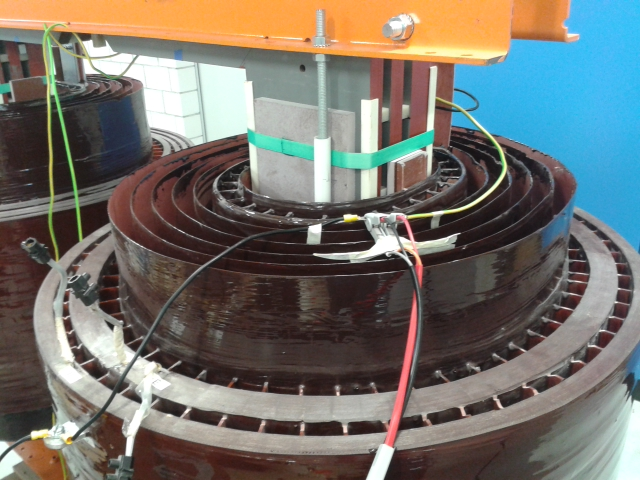
\includegraphics[width=0.5\textwidth]{./Trafo/images/resibloc.jpg}
	\caption{Resibloc-Testtransformator der Firma ABB. Zwischen den Layern ist der Luftspalt zur Kühlung ersichtlich.}
	\label{trafo:resibloc}
\end{figure}
Fr"uher wurde ein Transformator oder allgemein ein elektronisches Betriebsmittel nach Erfahrungen gebaut. Dabei war es gang und g"abe, dass mehrere Prototypen notwendig waren, bis die ersten Spannungspr"ufungen bestanden werden konnten. Deshalb sind CAD-Simulationen wesentlich schneller und vor allem kosteng"unstiger. Das Ziel soll es sein, den Transformator m"oglichst genau darzustellen und dessen Spannungsverteilung zu berechnen, denn die Spannung und die Geometrie zusammen ergeben das elektrische Feld, welches schlussendlich zu Durchschl"agen oder Teilentladungen f"uhrt.

An der Hochschule f"ur Technik Rapperswil wurde am Institut f"ur Energietechnik eine Methode entwickelt, wie die Spannungsverteilung bei einem Blitzstoss m"oglichst genau simuliert werden kann \cite{trafo:BILImpulse}. Diese Methode funktioniert sehr gut f"ur Leistungstransformatoren und konnte mit Messungen auch verifiziert werden. 
Soll dieses Prinzip aber auf Instrumententransformatoren angewendet werden, ergibt die wesentlich h"ohere Anzahl von Wicklungen und deren engeren Lagen nummerische Probleme mit dem momentanen L"osungsverfahren. 

Diese Probleme werden in diesem Abschnitt schrittweise behandelt und bestm"oglichst gel"ost. 


\subsection{Ersatzschaltbild}
Ein Transformator, ob "ol- oder luftgek"uhlt, kann prinzipiell mit dem Ersatzschaltbild \ref{trafo:einfaches_ESB} dargestellt werden. Dies macht Sinn, wenn der Transformator als Ganzes dargestellt werden will. Soll hingegen die Spannung an jeder Wicklung berechnet werden, kann dieses bereits bekannte, jedoch zu simple Ersatzschaltbild nicht verwendet werden. Es gilt nun, ein neues und genaueres Ersatzschaltbild zu finden. 

\begin{figure}
	\centering
	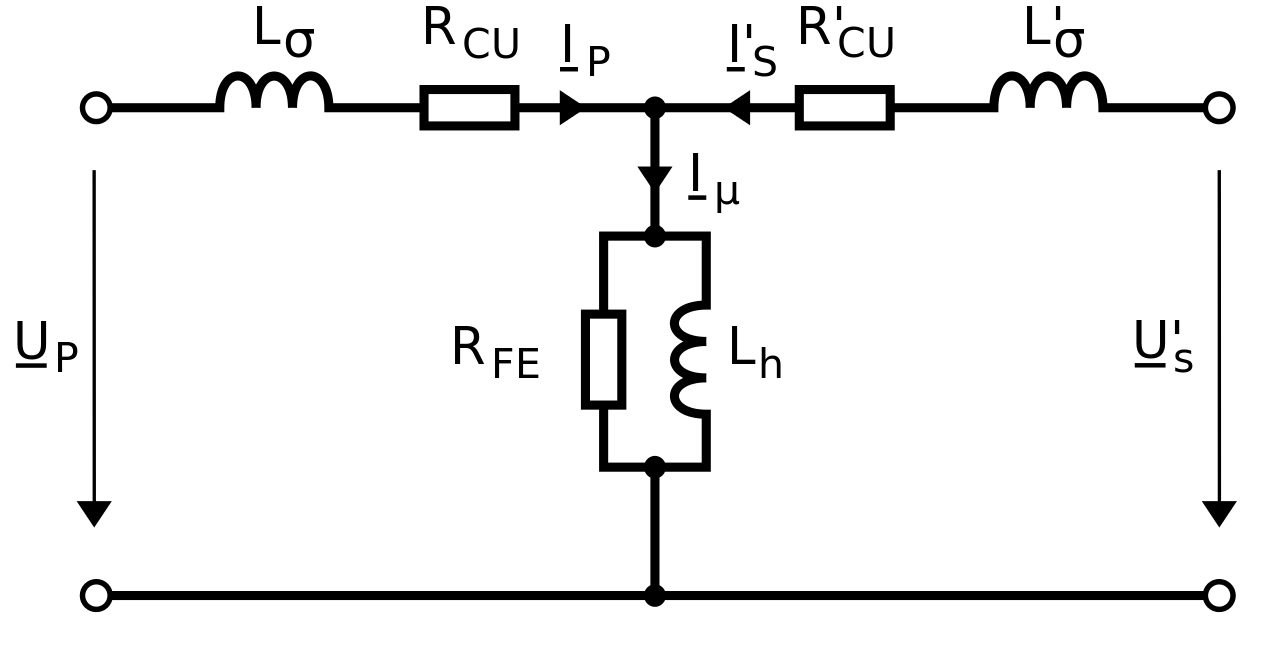
\includegraphics[width=0.5\textwidth]{./trafo/images/Einfaches_ESB.png}
	\caption[Einfaches Ersatzschaltbild f"ur einen Transformator]{Einfach Ersatzschaltbild f"ur einen Transformator.}
	\label{trafo:einfaches_ESB}
\end{figure}

Ein Ansatz ist es, jede Wicklung einzeln zu modellieren. Pro Windung wird ein elektrischer Widerstand sowie eine Induktivit"at in Serie geschaltet. Ebenfalls m"ussen die Kapazit"aten sowie die Leitf"ahigkeiten gegen"uber Masse und den "ubrigen Windungen ber"ucksichtigt werden \cite{trafo:BILImpulse}. 

Dieses Ersatzschaltbild wird in der Abbildung \ref{trafo:erweitertes_ESB} dargestellt. Als Veranschaulichung wird ein kleines Transformator-Beispiel, bestehend aus 4 Windungen, verwendet. Mit Messungen an Testtransformatoren zeigte sich, dass ab ca. 20 Windungen die Simulationen mit diesem Ersatzschaltbild sehr genau "ubereinstimmen. 

\begin{figure}
	\centering
	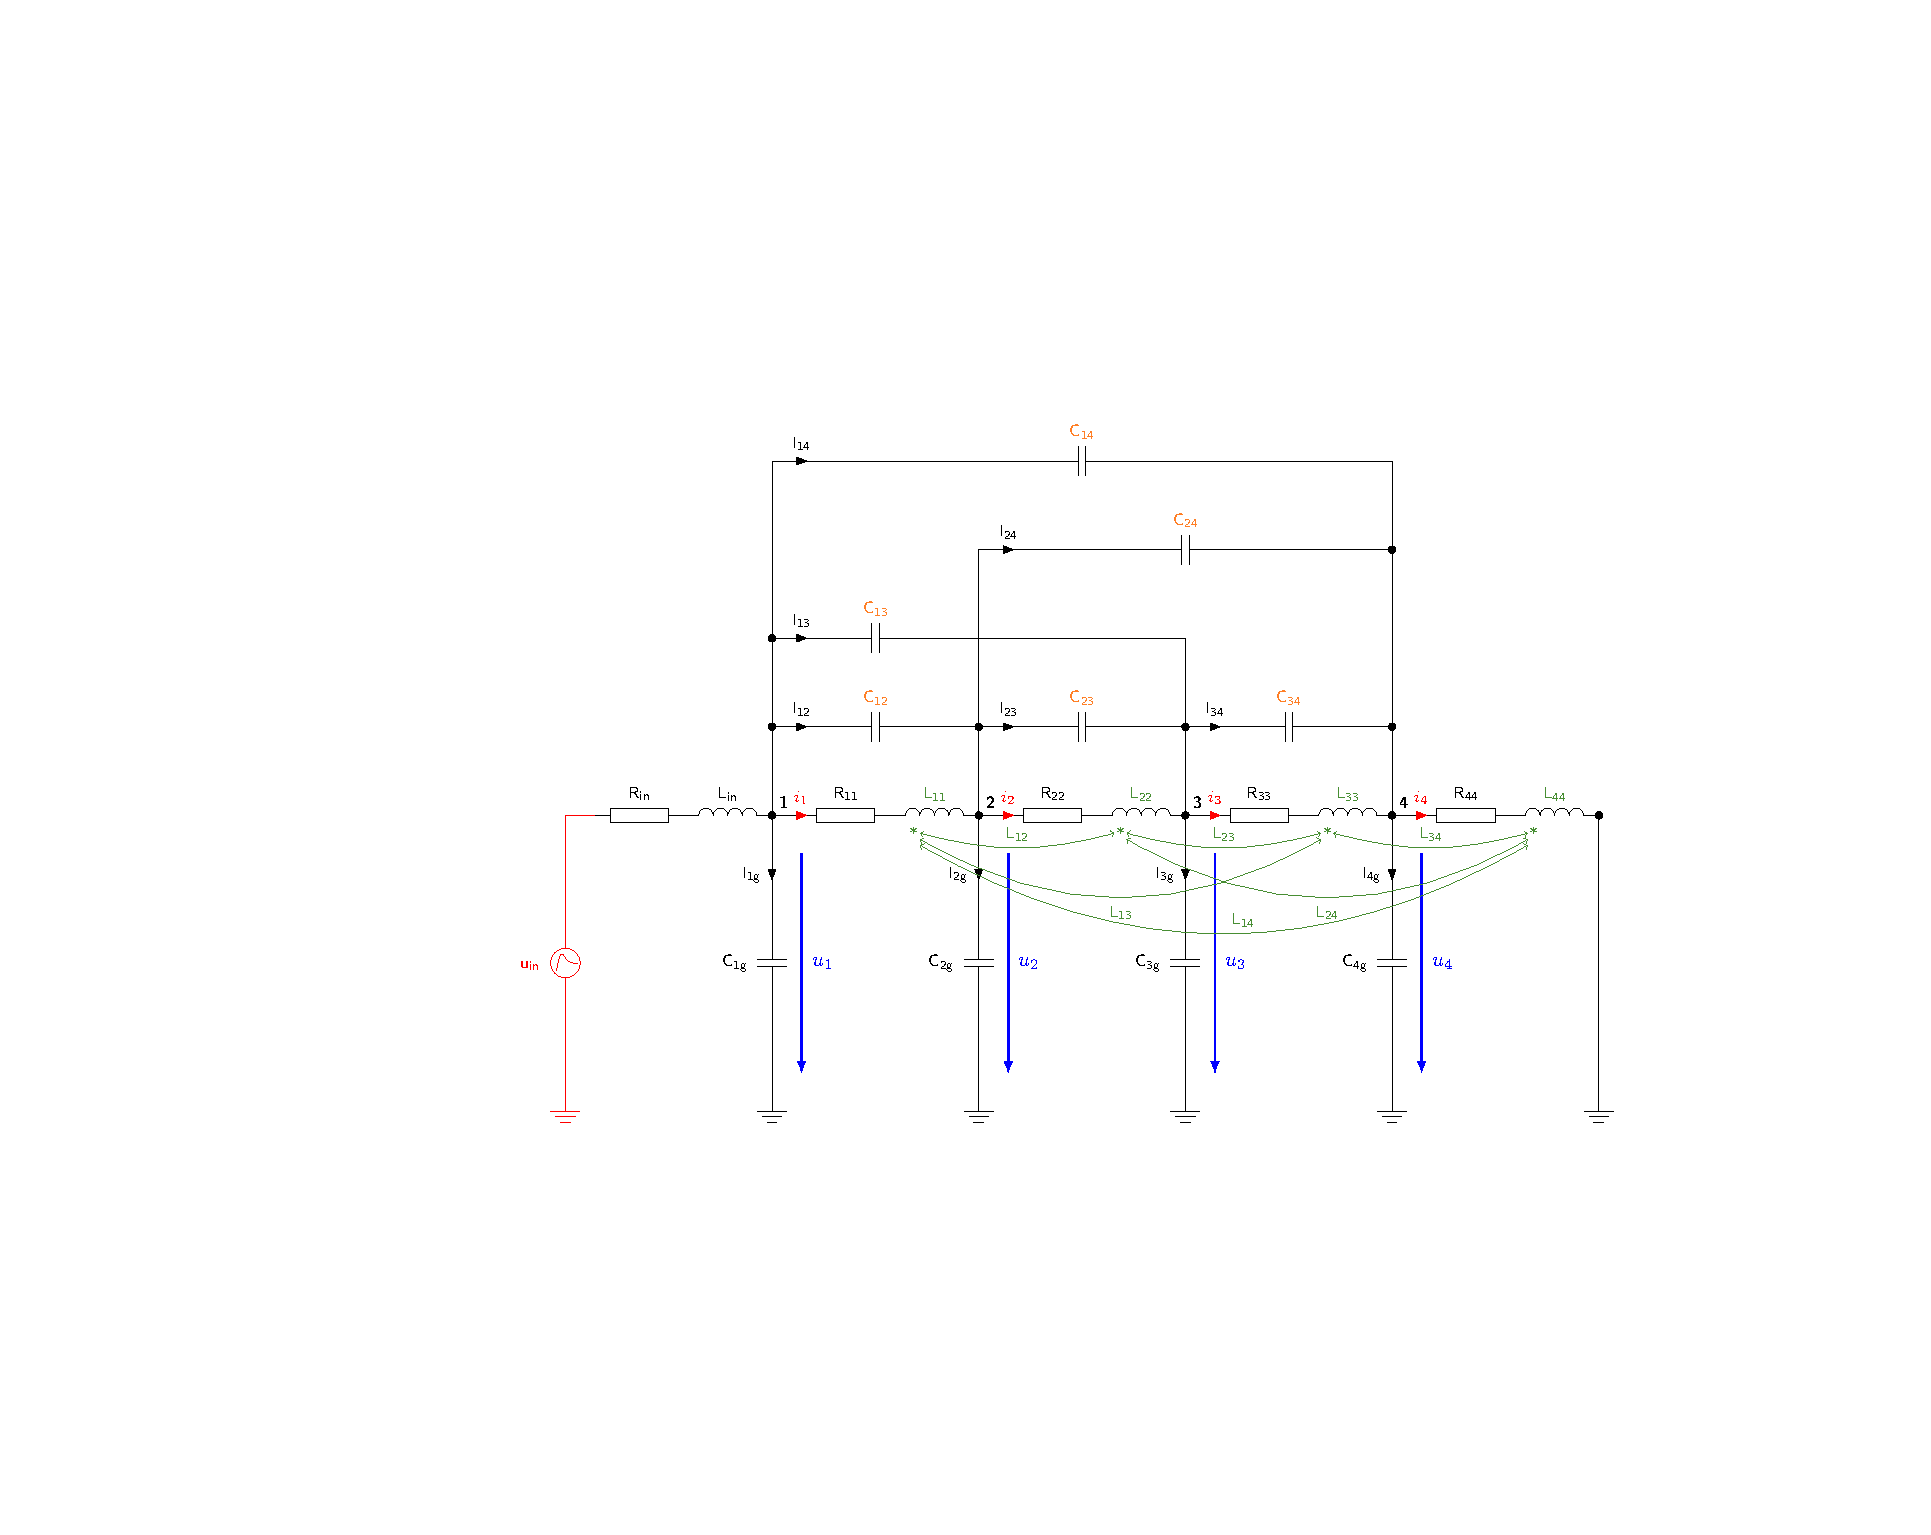
\includegraphics[width=\hsize]{./trafo/images/Trafo_Modell.pdf}
	\caption[Erweitertes Ersatzschaltbild f"ur einen Transformator]{Erweitertes Ersatzschaltbild f"ur einen Transformator mit 4 Wicklungen. Die Leitwerte zwischen den Wicklungen und gegen"uber Masse sind auf Grund der "Ubersichtlichkeit weggelassen worden. Die gr"unen Pfeile stellen die Mitkopplung, das heisst die Str"ome welche durch das Eigenfeld einer Windung in die anderen Windungen induziert wird, der Spulen dar. }
	\label{trafo:erweitertes_ESB}
\end{figure}

Damit die Werte der einzelnen Elementen ermittelt werden k"onnen, sind Finite-Element-Methode-(FEM)-Simulationen in einem CAD-Programm notwendig. Das Simulationsmodell im CAD-Programm des Transformators besteht aus in sich geschlossenen Windungen. Weil ein Transformator rotationssymmetrisch ist, kann auf eine rechenintensive 3D Feldsimulation verzichtet werden. Ein Beispiel eines Transformators ist in den Abbildungen \ref{trafo:infolytica} dargestellt.

\begin{figure}
	\centering    
	\subfigure[Ganzer Transformator]{
		\label{fig:a}
		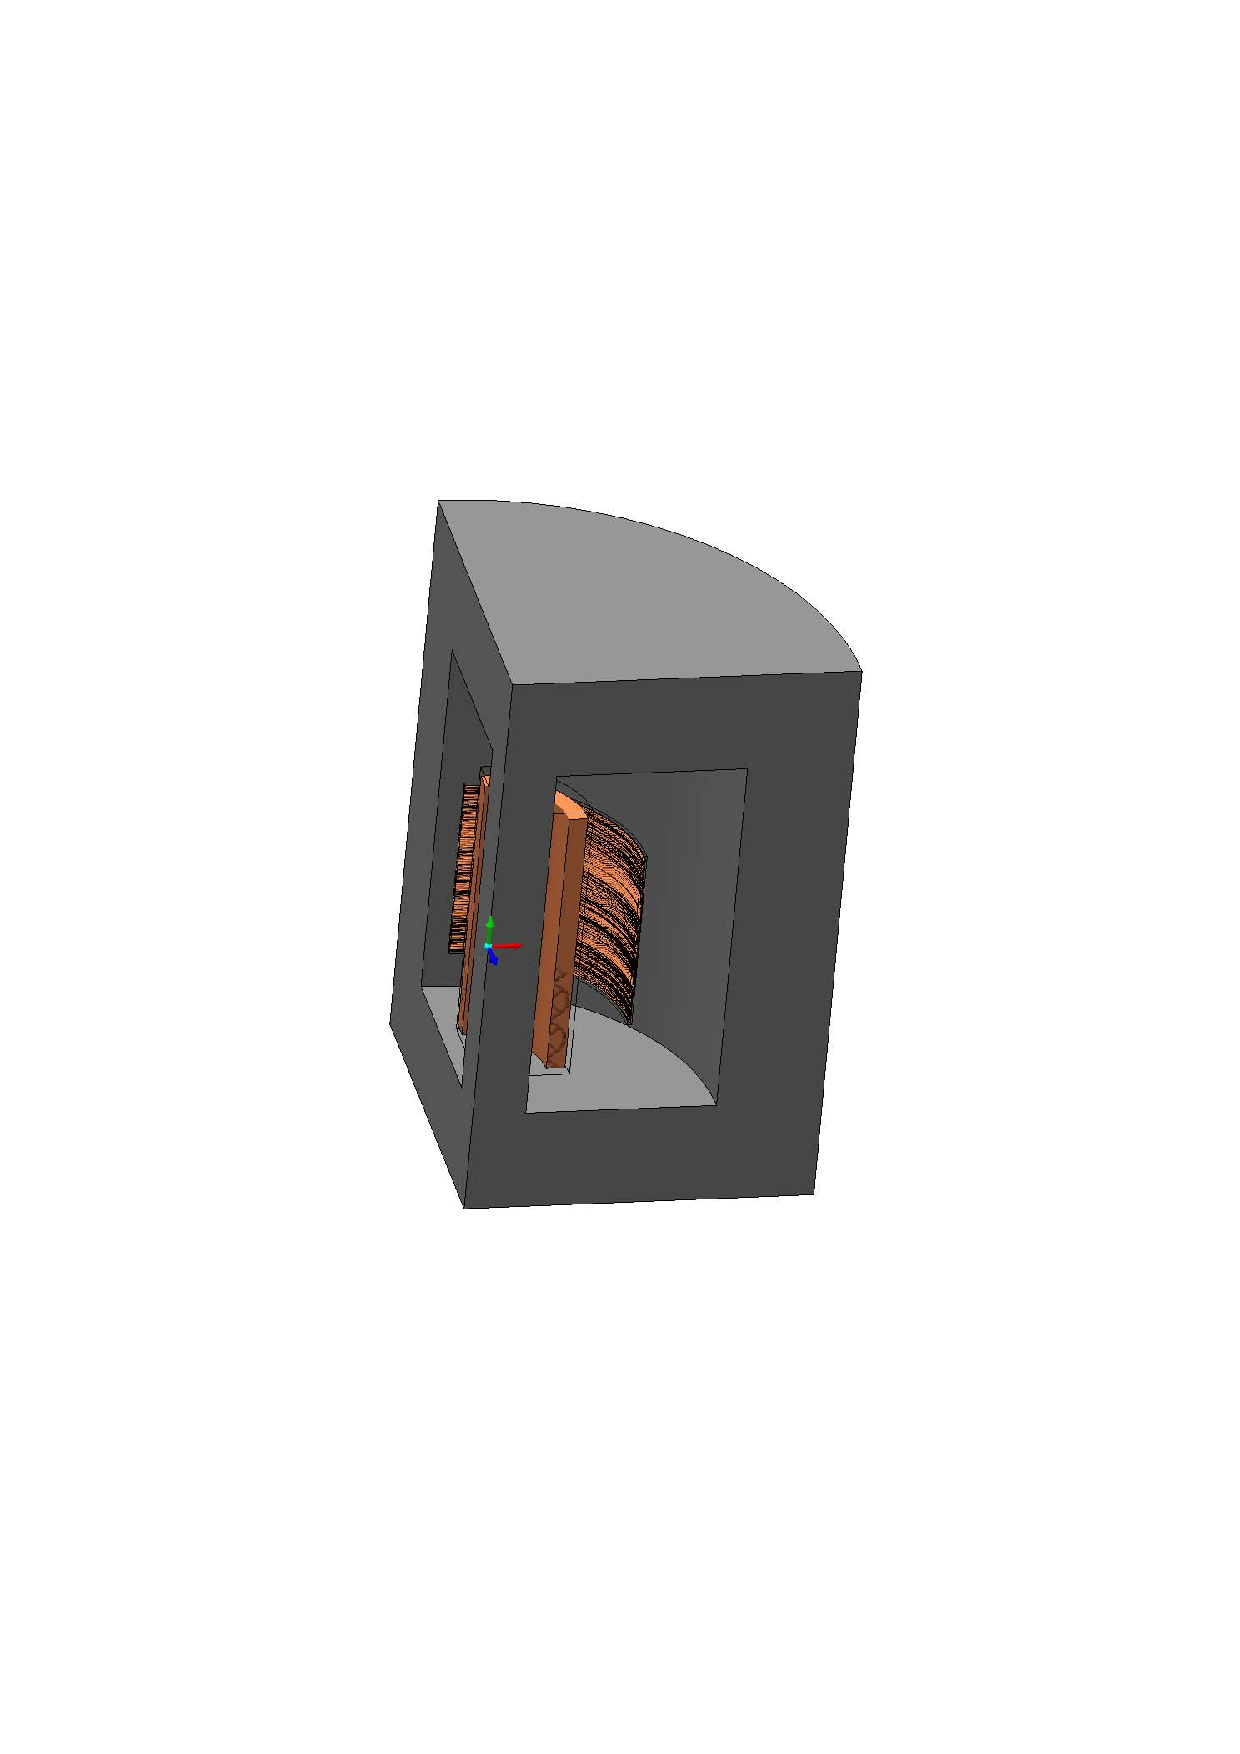
\includegraphics[height=6cm]{./Trafo/images/infolytica_ganzer_trafo.pdf}}
	\subfigure[Hochspannungwicklung]{
		\label{fig:b}
		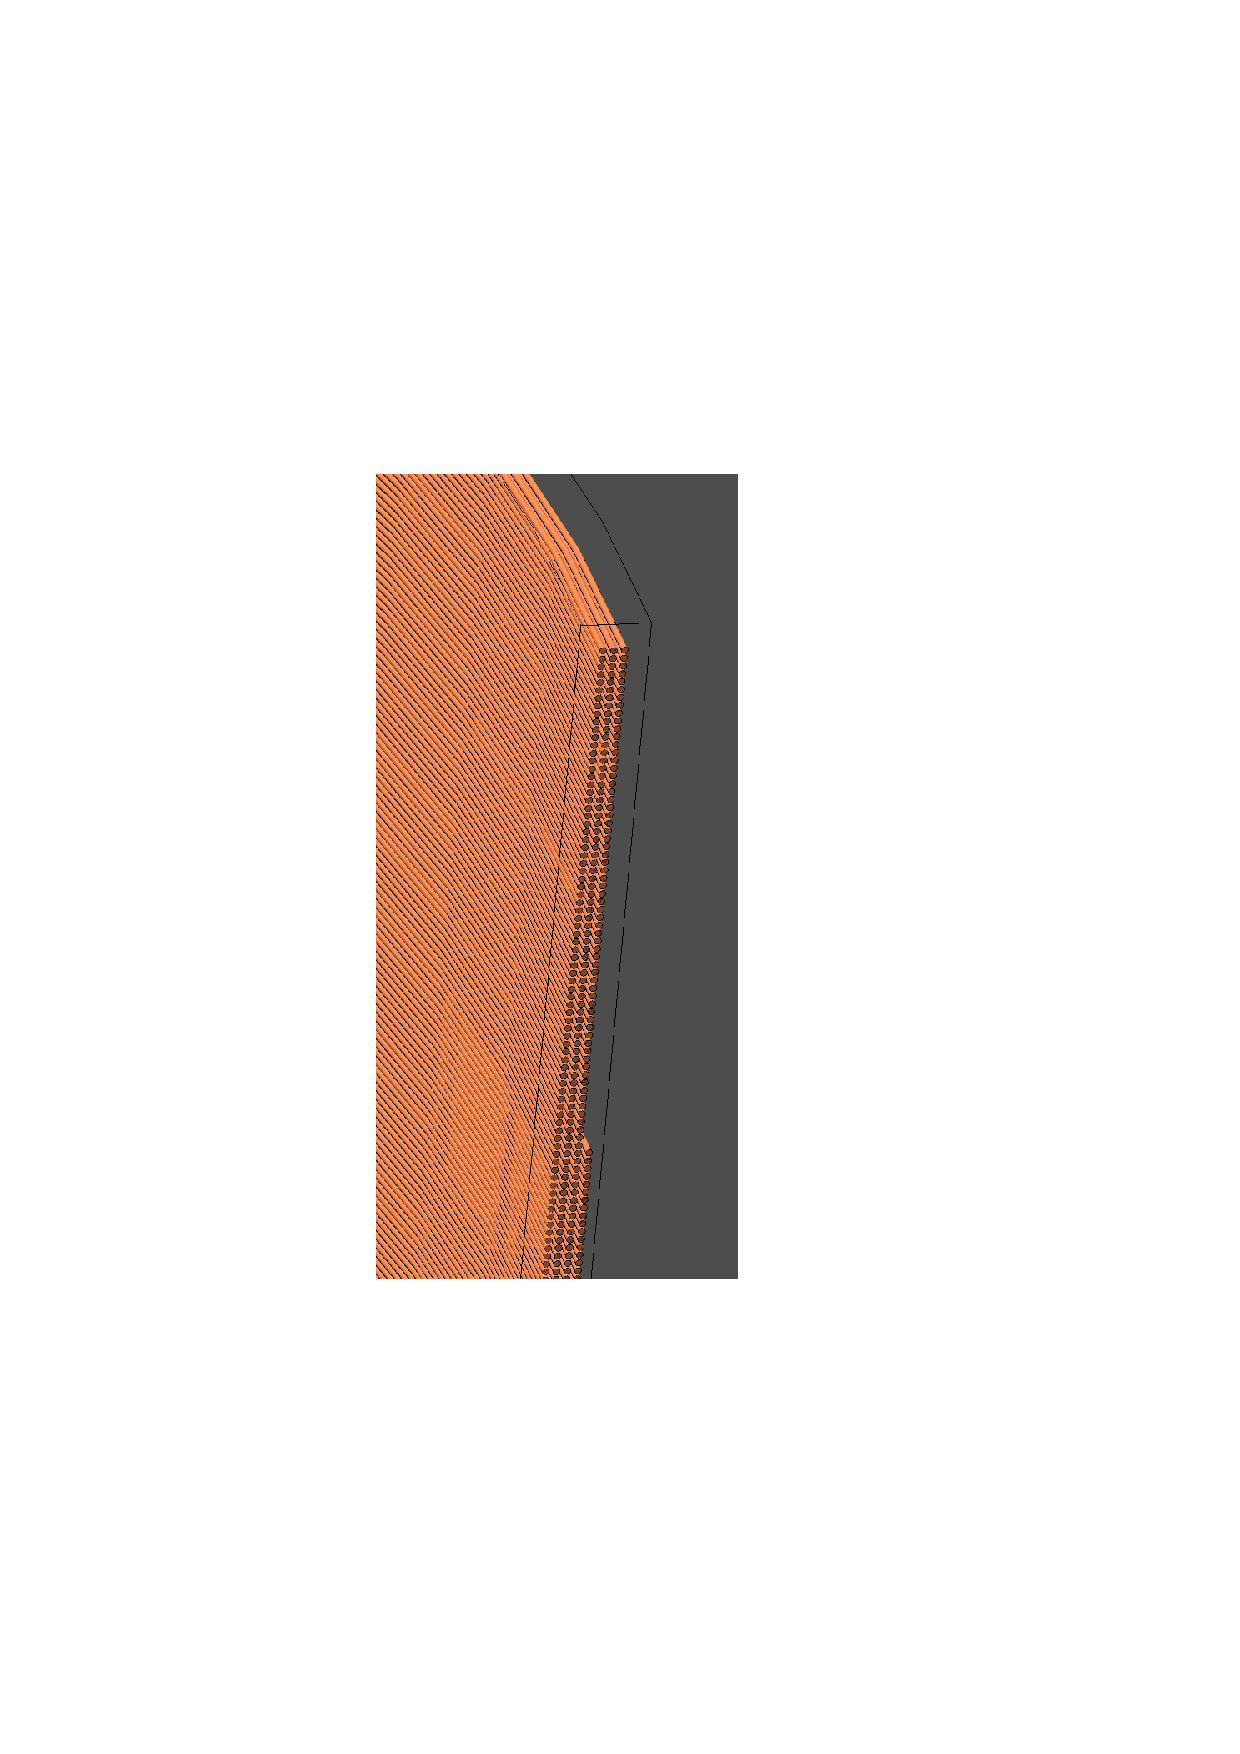
\includegraphics[height=6cm]{./Trafo/images/infolytica_windungen.pdf}}
	\caption{Darstellung eines rotationssymmetrischen Transformator in einem CAD-Programm. In \ref{fig:a} ist der ganze Transformator und in \ref{fig:b} ein Ausschnitt der Hochspannungswicklung abgebildet. Jede Windung ist für sich geschlossen moduliert.}
	\label{trafo:infolytica}
\end{figure}

Alle Windungen, abgesehen von einer, werden auf das Spannungspotential \SI{0}{\volt} gesetzt. Die aktuelle gemessene Wicklung wird hingegen auf das Potential von \SI{1}{\volt} gesetzt und anschliessend werden die Induktivit"aten sowie Kapazit"aten gegen"uber allen anderen Wicklungen berechnet. Dieser Vorgang wird für jede Windung wiederholt, bis alle Ersatzparameter für das Modell, und ins besonders für das Differentialgleichungssystem \ref{trafo:DGL}, bestimmt sind.

\subsection{Blitzstoss (\textbf{B}asic \textbf{I}nsulation \textbf{L}evel)}
Als Testspannung wird ein Blitzstoss wie in Abbildung \ref{trafo:BIL} verwendet. Mit diesem Spannungsimpuls soll die Spannungsfestigkeit bei einem Blitzeinschlag geprüft werden. Nach Norm muss die Anstiegszeit \SI{1.2}{\micro \second} und die Halbwertsababfallszeit (die Zeit, in welcher die Spannung auf \SI{50}{\percent} absinkt) \SI{50}{\micro \second} betragen. Die Höhe der Amplitude wird je nach Betriebsspannung in Kategorien eingeteilt, grundsätzlich beträgt sie aber ungefähr dem 6-fachen der Nennbetriebsspannung. Für die Berechnung wird auf Grund der Linearität meistens \SI{1}{\volt}, oder auch \textit{pro Einheit} (engl. \textit{per unit} [p.u.]), verwendet. 

\begin{figure}
	\centering
	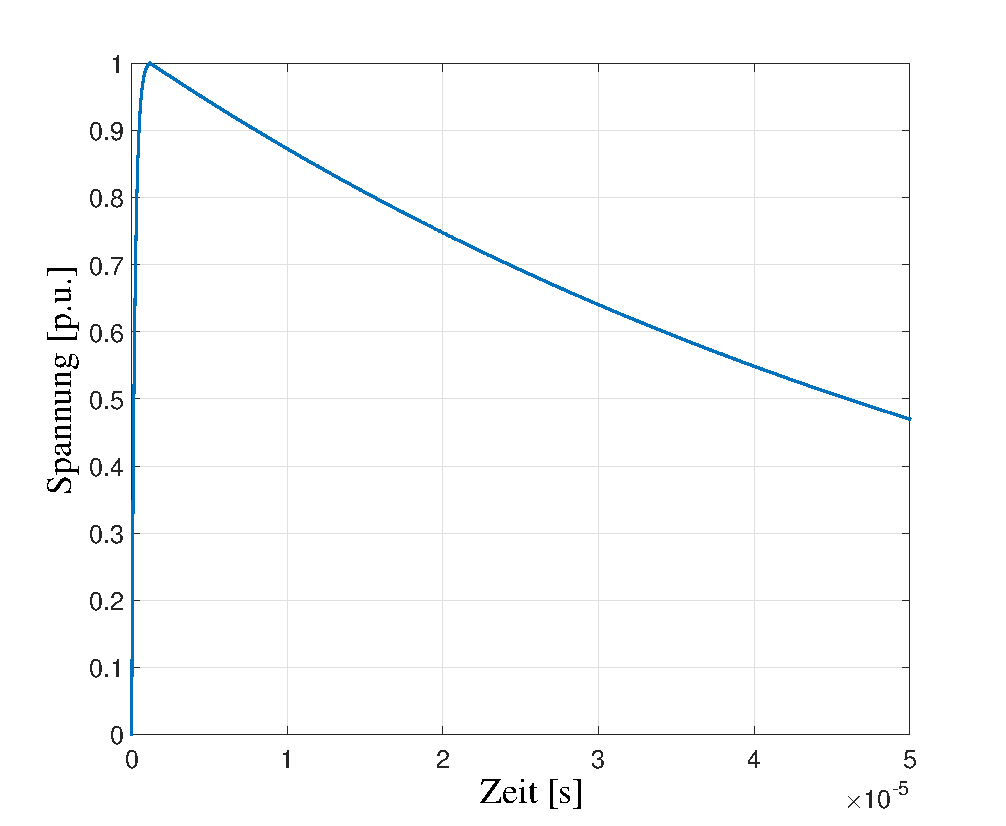
\includegraphics[width=0.6\textwidth]{./Trafo/images/pulse.pdf}
	\caption{Normierte Blitzstossspannung zur Testung der Durchschlagsfestigkeit.}
	\label{trafo:BIL}
\end{figure}

\section{Mathematische L"osung}
\subsection{Differentialgleichung}

Nun gilt es, eine Differentialgleichung f"ur das gefundene Ersatzschaltbild aufzustellen. Mittels dem Maschensatz (blaue Pfeile) und der Knotenpunktregel (rote Punkte) k"onnen die Differentialgleichungen pro Wicklung aufgestellt werden (dargestellt in \ref{trafo:orig}).

\begin{figure}
	\centering
	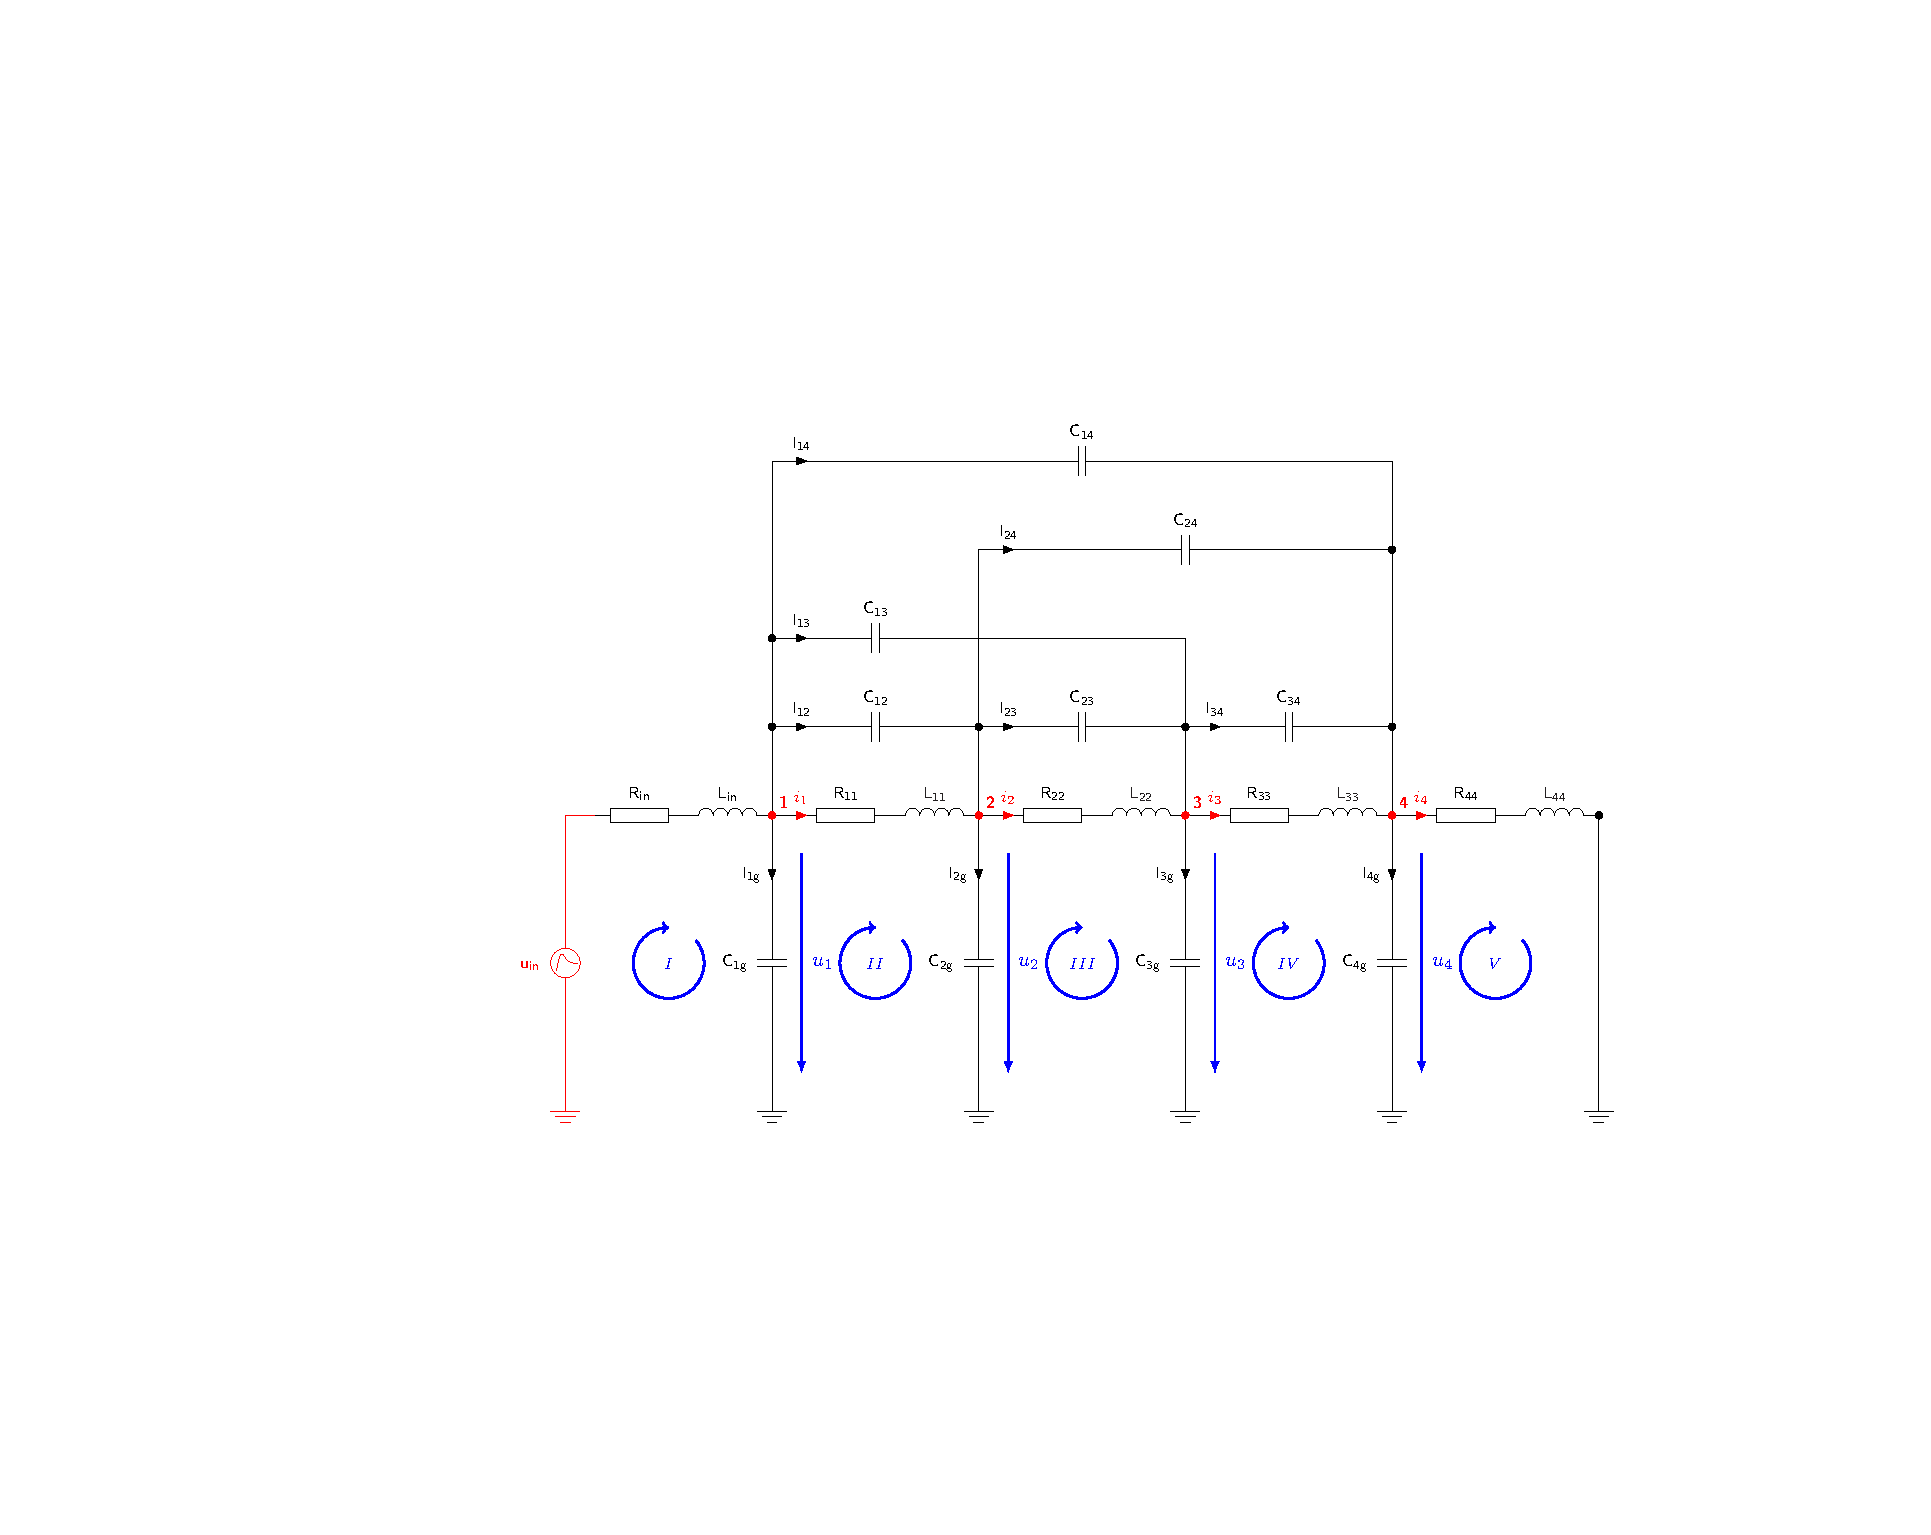
\includegraphics[width=\hsize]{./trafo/images/orig_trafo.pdf}
	\caption[Erweitertes Ersatzschaltbild f"ur einen Transformator mit Maschensatz und Knotenpunkt]{Erweitertes Ersatzschaltbild f"ur einen Transformator mit 4 Wicklungen. Die blauen Pfeil stellen den Maschensatz und die roten Punkte die Knotenpunktregel dar.}
	\label{trafo:orig}
\end{figure}

Beispielsweise kann die Gleichungen der Wicklung 1 als 

\begin{equation*}
	u_\mathrm{Rin} + u_\mathrm{Lin} + u_1 = u_\mathrm{in}
\end{equation*}
und 
\begin{equation}
	i_\mathrm{in} = i_1 + i_{C1g} + i_{R12} + i_{C12} + i_{R13} + i_{C13} + i_{R14} + i_{C14}
\end{equation}
geschrieben werden. 

Mit einigen Umformungen kann der ganze Transformator als System mehreren Differentialgleichungen geschrieben werden \cite{trafo:SeminarCHR}. Als Beispiel wird wiederum der Transformator mit 4 Windungen gew"ahlt. Der Vektor $E$ ist der St"orterm des Systems, welcher in diesem Falle der Blitzstoss ist.

{\footnotesize 
\begin{align}
			&
			\underbrace{\begin{bmatrix}
			L_\mathrm{in}&0&0&0&0 & 0&0&0&0 \\
			0&L_{11}&L_{12}&L_{13}&L_{14} & 0&0&0&0 \\
			0&L_{21}&L_{22}&L_{23}&L_{24} & 0&0&0&0 \\
			0&L_{31}&L_{32}&L_{33}&L_{34} & 0&0&0&0 \\
			0&L_{41}&L_{42}&L_{43}&L_{44} & 0&0&0&0 \\
			0&0&0&0&0 & \sum{C_{1\mathrm{x}}}&-C_{12}&-C_{13}&-C_{14} \\
			0&0&0&0&0 & -C_{21}&\sum{C_{2\mathrm{x}}}&-C_{23}&-C_{24} \\
			0&0&0&0&0 & -C_{31}&-C_{32}&\sum{C_{3\mathrm{x}}}&-C_{34} \\
			0&0&0&0&0 & -C_{41}&-C_{42}&-C_{43}&\sum{C_{4\mathrm{x}}}
			    \end{bmatrix}}_{\text{$M$}}
			\cdot
			\underbrace{\begin{bmatrix}
			\frac{di_\mathrm{in}}{dt} \\
			\frac{di_1}{dt} \\
			\frac{di_2}{dt} \\
			\frac{di_3}{dt} \\
			\frac{di_4}{dt} \\
			\frac{du_1}{dt} \\
			\frac{du_2}{dt} \\
			\frac{du_3}{dt} \\
			\frac{du_4}{dt}
			\end{bmatrix}}_{\text{$\dot{x}$}}
			= \nonumber \\
			&
			\underbrace{\begin{bmatrix}
			-R_\mathrm{in}&0&0&0&0 & -1&0&0&0 \\
			0&-R_{11}&0&0&0 & 1&-1&0&0 \\
			0&0&-R_{22}&0&0 & 0&1&-1&0 \\
			0&0&0&-R_{33}&0 & 0&0&1&-1 \\
			0&0&0&0&-R_{44} & 0&0&0&1 \\
			1&-1&0&0&0 & -\sum G_{1\mathrm{x}}&G_{12}&G_{13}&G_{14} \\
			0&1&-1&0&0 & G_{21} &- \sum G_{2\mathrm{x}}& G_{23}& G_{24} \\
			0&0&1&-1&0 & G_{31} & G_{32} &-\sum G_{3\mathrm{x}}&G_{34} \\
			0&0&0&1&-1 & G_{41}&G_{42}&G_{43}&-\sum G_{4\mathrm{x}}
			\end{bmatrix}}_{\text{$N$}}
			\cdot
			\underbrace{\begin{bmatrix}
			i_\mathrm{in} \\
			i_1 \\
			i_2 \\
			i_3 \\
			i_4 \\
			u_1 \\
			u_2 \\
			u_3 \\
			u_4
			\end{bmatrix}}_{\text{$x$}}
			+
			\underbrace{\begin{bmatrix}
			u_\mathrm{in} \\
			0 \\
			0 \\
			0 \\
			0 \\
			0 \\
			0 \\
			0 \\
			0
			\end{bmatrix}}_{\text{$E$}}
			\label{trafo:DGL}
\end{align}
}
		


Die Matrix $M$ ist eine symmetrische Matrix, was f"ur weitere Berechnungen wesentliche Vorteile mit sich bringt. Die Matrix $N$ ist fast symmetrisch. Wenn der Maschensatz jedoch in die andere Richtung als in Abbildung \ref{trafo:orig} angewendet wird, l"asst sich auch diese Matrix mit sehr geringem Aufwand in die symmetrische Form bringen. Dies ist f"ur dieses Beispiel zwar nicht n"otig, trotzdem kann es f"ur andere L"osungsans"atze von Vorteil sein. Aus der Gleichung \ref{trafo:DGL} wird nun 

{\footnotesize 
\begin{align}
			&
			\underbrace{\begin{bmatrix}
			\color{red}-\color{black}L_\mathrm{in}&0&0&0&0 & 0&0&0&0 \\
			0&\color{red}-\color{black}L_{11}&\color{red}-\color{black}L_{12}&\color{red}-\color{black}L_{13}&\color{red}-\color{black}L_{14} & 0&0&0&0 \\
			0&\color{red}-\color{black}L_{21}&\color{red}-\color{black}L_{22}&\color{red}-\color{black}L_{23}&\color{red}-\color{black}L_{24} & 0&0&0&0 \\
			0&\color{red}-\color{black}L_{31}&\color{red}-\color{black}L_{32}&\color{red}-\color{black}L_{33}&\color{red}-\color{black}L_{34} & 0&0&0&0 \\
			0&\color{red}-\color{black}L_{41}&\color{red}-\color{black}L_{42}&\color{red}-\color{black}L_{43}&\color{red}-\color{black}L_{44} & 0&0&0&0 \\
			0&0&0&0&0 & \sum{C_{1\mathrm{x}}}&-C_{12}&-C_{13}&-C_{14} \\
			0&0&0&0&0 & -C_{21}&\sum{C_{2\mathrm{x}}}&-C_{23}&-C_{24} \\
			0&0&0&0&0 & -C_{31}&-C_{32}&\sum{C_{3\mathrm{x}}}&-C_{34} \\
			0&0&0&0&0 & -C_{41}&-C_{42}&-C_{43}&\sum{C_{4\mathrm{x}}}
			    \end{bmatrix}}_{\text{$M$}}
			\cdot
			\underbrace{\begin{bmatrix}
			\frac{di_\mathrm{in}}{dt} \\
			\frac{di_1}{dt} \\
			\frac{di_2}{dt} \\
			\frac{di_3}{dt} \\
			\frac{di_4}{dt} \\
			\frac{du_1}{dt} \\
			\frac{du_2}{dt} \\
			\frac{du_3}{dt} \\
			\frac{du_4}{dt}
			\end{bmatrix}}_{\text{$\dot{x}$}}
			= \nonumber \\
			&
			\underbrace{\begin{bmatrix}
			\color{red}+\color{black}R_\mathrm{in}&0&0&0&0 & \color{red}+\color{black}1&0&0&0 \\
			0&\color{red}+\color{black}R_{11}&0&0&0 & \color{red}-\color{black}1&\color{red}+\color{black}1&0&0 \\
			0&0&\color{red}+\color{black}R_{22}&0&0 & 0&\color{red}-\color{black}1&\color{red}+\color{black}1&0 \\
			0&0&0&\color{red}+\color{black}R_{33}&0 & 0&0&\color{red}-\color{black}1&\color{red}+\color{black}1 \\
			0&0&0&0&\color{red}+\color{black}R_{44} & 0&0&0&\color{red}-\color{black}1 \\
			1&-1&0&0&0 & -\sum G_{1\mathrm{x}}&G_{12}&G_{13}&G_{14} \\
			0&1&-1&0&0 & G_{21} &- \sum G_{2\mathrm{x}}& G_{23}& G_{24} \\
			0&0&1&-1&0 & G_{31} & G_{32} &-\sum G_{3\mathrm{x}}&G_{34} \\
			0&0&0&1&-1 & G_{41}&G_{42}&G_{43}&-\sum G_{4\mathrm{x}}
			\end{bmatrix}}_{\text{$N$}}
			\cdot
			\underbrace{\begin{bmatrix}
			i_\mathrm{in} \\
			i_1 \\
			i_2 \\
			i_3 \\
			i_4 \\
			u_1 \\
			u_2 \\
			u_3 \\
			u_4
			\end{bmatrix}}_{\text{$x$}}
			\color{red}-\color{black}
			\underbrace{\begin{bmatrix}
			u_\mathrm{in} \\
			0 \\
			0 \\
			0 \\
			0 \\
			0 \\
			0 \\
			0 \\
			0
			\end{bmatrix}}_{\text{$E$}}
			\label{trafo:symmetricalDGL}
\end{align}
}

Dieses System mehrerer Differentialgleichungen kann auch mit Matrizen und Vektoren geschrieben werden, welches sich etwas "ubersichtlicher darstellen l"asst. 

\begin{equation}
	M \dot x = N x + E
	\label{trafo:matricesDGL}
\end{equation}

Wird die Massenmatrix $M$ auf die rechte Seite der Gleichung \ref{trafo:matricesDGL} dividiert, ergibt dies

\begin{equation}
	\dot{x} = M^{-1}N x + M^{-1} E = A x + B
\end{equation}
welches die allgemein bekannte und auch l"osbare Zustandsraumdarstellung \index{Zustandsraumdarstellung} (engl. state space) ist.

Das Problem scheint bereits gel"ost zu sein, wenn sich die Massenmatrix $M$ invertieren l"asst. In der Theorie w"are dies tats"achlich auch machbar, jedoch sehr aufw"andig. Weil auch gewisse Eigenwerte zu klein sind, explodiert die L"osung und kann somit mit diesem Ansatz nicht gel"ost werden.

Folglich muss ein Ansatz gefunden werden, welcher die Massenmatrix $M$ m"oglichst ressourcenschonend invertiert und bei der Inversion der Eigenwerte die L"osung stabil bleibt. 


\subsection{Singular Value Decomposition (SVD) \index{Singular Value Decomposition}}
Eine M"oglichkeit stellt die Singular Value Decomposition, zu Deutsch Singul"arwertzerlegung, dar. Ohne Gedanken "uber die Dimensionen der Matrix $M$ zu verlieren, wird der SVD-Satz verwendet \cite{trafo:Watkins}. 

\begin{satz}
	\label{trafo:SVDTheorem}
	(\textit{SVD Theorem}) Sei $M\in \mathbb{R}^{n \times m}$ eine besetzte Matrix mit Rang $r$. Dann kann $M$ als Produkt
	\begin{equation}
		M = USV^\top
		\label{trafo:svd}
	\end{equation} 
	geschrieben werden, wobei $U \in \mathbb{R}^{n \times n}$ und $V \in \mathbb{R}^{m \times m}$ orthogonal sind und $S \in \mathbb{R}^{n \times m}$ eine rechteckige Diagonalmatrix ist 
	\begin{equation*}
		S = \left( 
			\begin{array}{ccc|ccc}
				\lambda_1 &          &          &        & \vdots &        \\
				& \ddots   &          & \cdots & 0      & \cdots \\
				&          & \lambda_r &        & \vdots &        \\
				\hline
				&  \vdots  &          &        & \vdots &        \\
				\cdots   &  0       & \cdots   & \cdots & 0      & \cdots \\
				&  \vdots  &          &        & \vdots &   \\				
				\end{array}
			\right) 
			\hspace{2cm}\lambda_1 \geq \lambda_2 \geq \dots \lambda_r > 0. 
	\end{equation*}
\end{satz}
F"ur die Herleitung und den Beweis des Satzes \ref{trafo:SVDTheorem} wird auf die Fachliteratur verwiesen \cite{trafo:Watkins}.

Einfach erkl"aren l"asst sich die Singul"arwertzerlegung mit jeweils zwei Rotationen, es sind dies die Matrizen $U$ und $V^\top$, und einer Streckung durch die Diagonalmatrix $S$. Dieser Vorgang ist in Abbildung \ref{trafo:SVDFig} dargestellt. 

Die Matrix $U$ besitzt in der senkrechte Eigenvektoren
\begin{equation*}
	\left( 
		\begin{array}{cccc}
		u_1 & u_2 & \dots & u_n  \\		
		\end{array}
	\right) 
\end{equation*}
und l"asst sich mit 
\begin{equation*}
	M M^\top = U S \underbrace{V^\top V}_{E} S^\top U^\top = U \underbrace{S S^\top}_{S^2} U
\end{equation*}
berechnen und anschliessend aufl"osen \cite{trafo:Watkins}. \color{red}TODO\color{black}

Die Matrix $V$ besitzt in der Vertikale Eigenvektoren
\begin{equation*}
	\left( 
		\begin{array}{c}
		{v_1}^{\top}\\
		{v_2}^{\top}\\
		\vdots\\
		{v_m}^{\top}\\			
		\end{array}
	\right) 
\end{equation*}
und l"asst sich mit 
\begin{equation*}
	M^\top M = V S^\top \underbrace{U^\top U}_{E} S V^\top = V \underbrace{S^\top S}_{S^2} V^\top 
\end{equation*}
berechnen und anschliessend aufl"osen \cite{trafo:Watkins}.

Als etwas schnellere Alternative kann die Berechnung von $V$ auch aus der Gleichung \ref{trafo:svd} erfolgen, denn $M$, $S$ und $U$ sind bekannt. 
\begin{align*}
	M^\top &= V \underbrace{S^\top}_{S} U^\top\\
	S^{-1} M^\top &= V U^\top\\
	V &= S^{-1} M^\top \left(U^\top\right) = S^{-1} M^\top U
\end{align*}

\begin{figure}
	\centering
	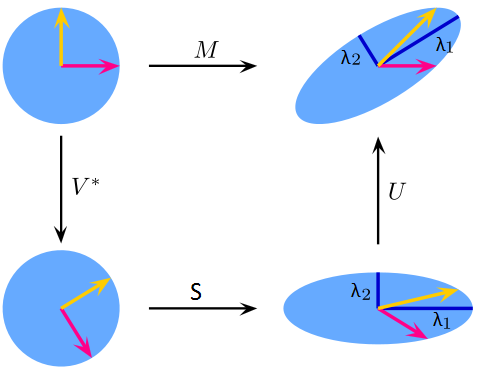
\includegraphics[width=0.4\textwidth]{./trafo/images/svd.png}
	\caption{Grafische Darstellung der Singul"arwertzerlegung \cite{trafo:SVDWiki}.}
	\label{trafo:SVDFig}
\end{figure}

Da es sich bei der Matrix $M$ um eine symmetrische Matrix handelt, sind die beiden Matrizen $U$ und $V$ im Betrag identisch. Falls die Eigenwerte der Matrix $M$ alle dasselbe Vorzeichen besitzen, sind die Matrizen $U$ und $V$ gar identisch. Weil ein Transformator physikalisch gesehen unbedingt eine D"ampfung haben muss, soll heissen alle Eigenwerte einen negative Realteil besitzen, gilt $U = V$. Dies kann auch nummerisch verifiziert werden.

\subsubsection{Unterdr"uckung von unerw"unschten Eigenwerten}
Die rechteckige Diagonalmatrix $S$ wird wegen der symmetrischen Matrix $M$ zu einer quadratischen Matrix. Dies bedeutet, dass sich auf der ganzen Diagonale Eigenwerte des Systems befinden. Ein Ansatz zur Unterdr"uckung unerw"unschten Frequenzen kann sein, zu kleine Eigenwerte $\lambda < tol$, welche in der Numerik 'explodieren' und physikalisch gesehen zu grosse und unm"ogliche Frequenzen sind, auf Null zu setzen. Dies ergibt die Diagonalmatrix 
\begin{equation*}
	S = \left( 
			\begin{array}{cccccc}
				\lambda_1 & & & & & \\
				& \ddots & & & &  \\
				& & \lambda_{tol} & & & \\
				& & & 0 & & \\
				& & & & \ddots & \\
				& & & & & 0 \\				
				\end{array}
			\right) 
			\hspace{2cm}\lambda_1 \geq \lambda_2 \geq \dots \lambda_{tol} > 0. 
\end{equation*}

\subsubsection{Inversion}
Als weiteres gilt es, eine einfache 'Inversion' der Matrix $M$ zu finden. Bis anhin wurde die Singul"arwertzerlegung angewendet, in der Annahme, schlussendlich eine Vereinfachung der Inversion zu finden. Die Inversion zeigt tats"achlich, dass sich einiges vereinfachen l"asst.
\begin{equation*}
	M^{-1} = \left(USV^\top\right)^{-1} = \left(V^\top\right)^{-1} S^{-1} U^{-1}
\end{equation*}
Da die Matrizen $U$ und $V$ symmetrisch sind, gilt $U^{-1} = U^\top$ und $\left(V^\top\right)^{-1} = V$. Dadurch kann die Gleichung als 
\begin{equation*}
	M^{-1} = V S^{-1} U^\top
\end{equation*}
geschrieben werden.

Dies ist wesentlich schneller zu berechnen als die Inverse der Matrix $M$, da lediglich die Diagonalmatrix invertiert werden muss.

\subsubsection{Implementation}
Die Implementation in Matlab l"asst sich sehr kompakt und elegant darstellen. Wie soeben erkl"art werden zu kleine Eigenwerte auf Null gesetzt und anschliessend die Inverse berechnet. 

{\scriptsize \lstinputlisting{./trafo/code/svd.m}}

\subsubsection{Resultate}
Damit der Wert der Toleranz bestimmt werden kann, m"ussen ein paar Testl"osungen erstellt werden. Als L"osungsverfahren wurde das etwas langsame, jedoch genaue nummerische Verfahren \texttt{ode45} von Matlab verwendet. In der Abbildung \ref{trafo:SVDTol} lassen sich die Unterschiede der gew"ahlten Toleranzen sehr gut erkennen. Wenn die Toleranzen $10^{-11}$ und $10^{-12}$ gew"ahlt werden, l"asst sich das Problem l"osen, jedoch ist das Verhalten des Systems erfahrungsgem"ass nicht ganz realistisch. Die L"osung mit der Toleranz $10^{-13}$ zeigt, wie es in der Praxis tats"achlich aussehen sollte. Wird die Toleranz hingegen noch einmal etwas verringert, explodiert die L"osung und ist somit nicht mehr brauchbar. Dieser Fall ist in Abbildung \ref{trafo:SVDTol} unten rechts dargestellt. Die y-Achse f"uhrt nummerisch von minus bis plus Unendlich.

	\begin{figure}
	    \centering
	    \begin{minipage}{.5\textwidth}
	        \centering
	        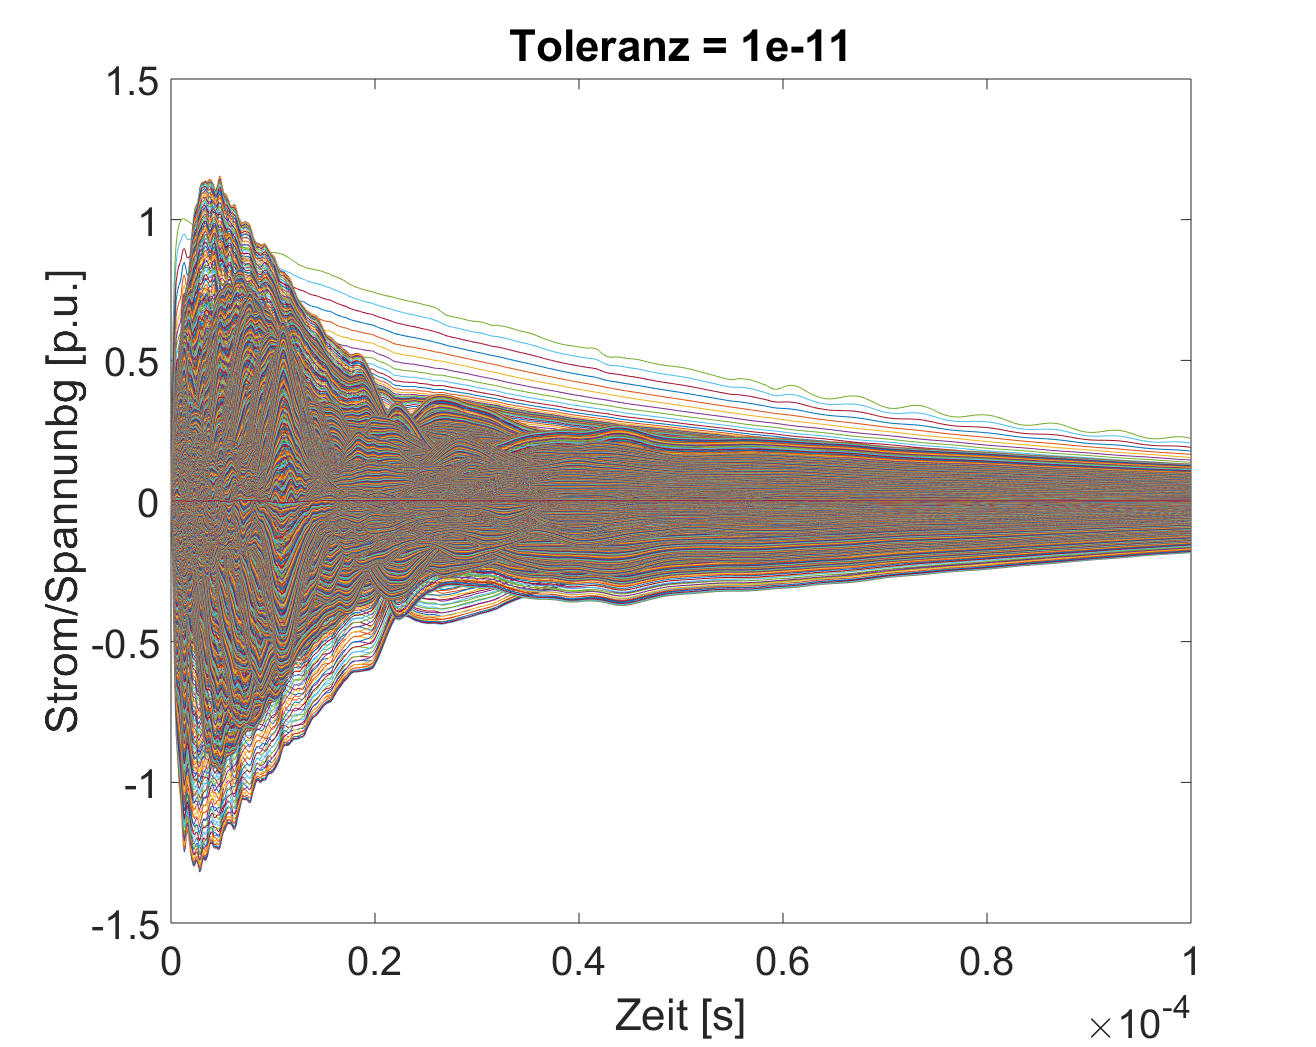
\includegraphics[width=\linewidth]{./trafo/images/svd11.png}
	    \end{minipage}%
	    \begin{minipage}{.5\textwidth}
	        \centering
	        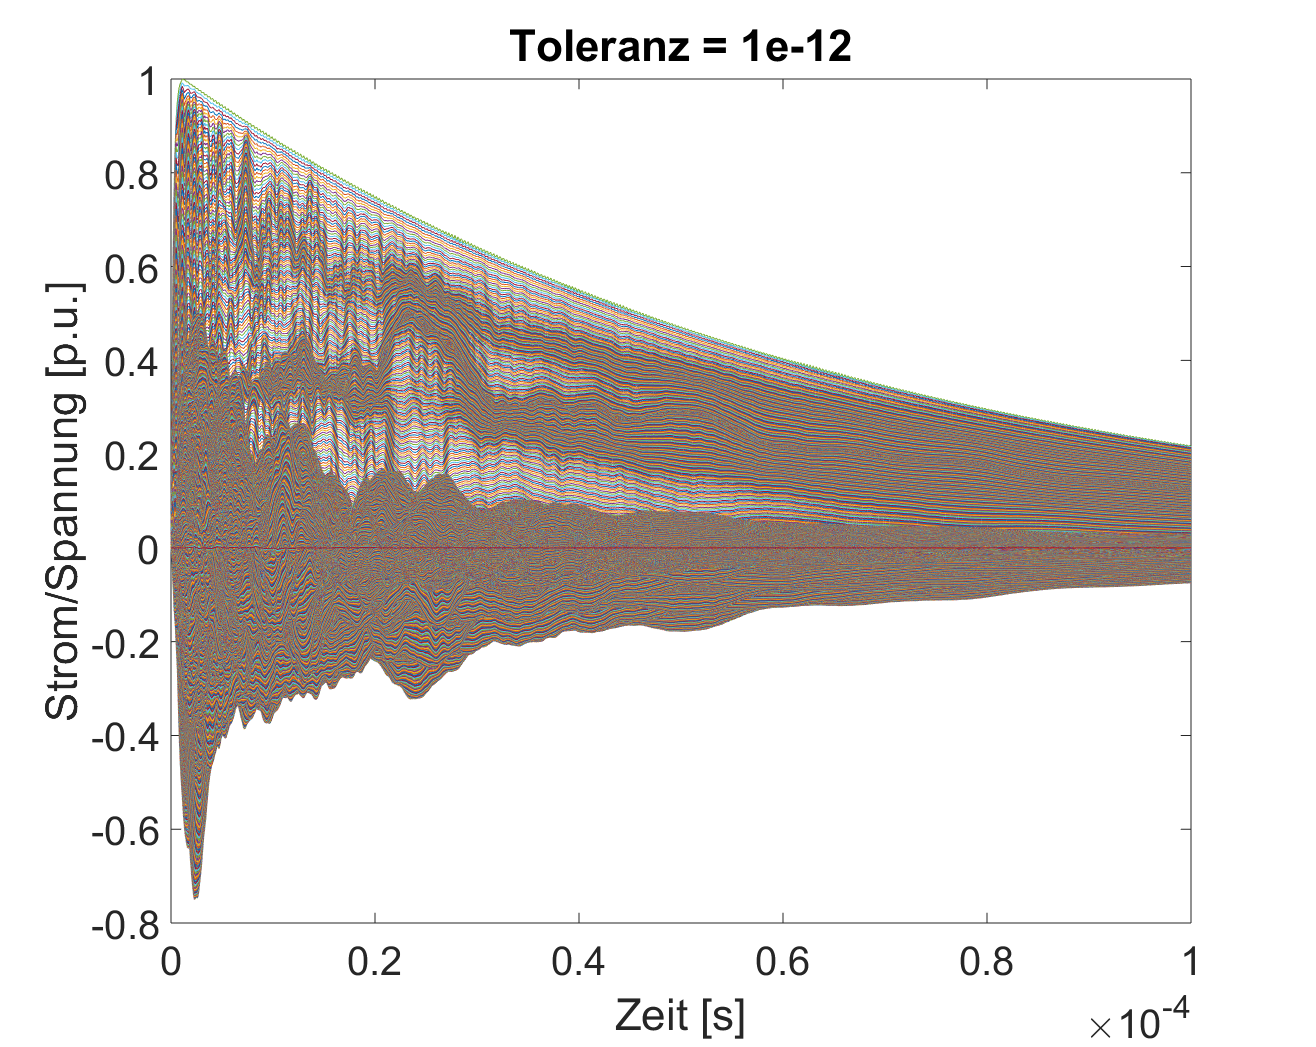
\includegraphics[width=\linewidth]{./trafo/images/svd12.png}
	    \end{minipage}
		\begin{minipage}{.5\textwidth}
	        \centering
	        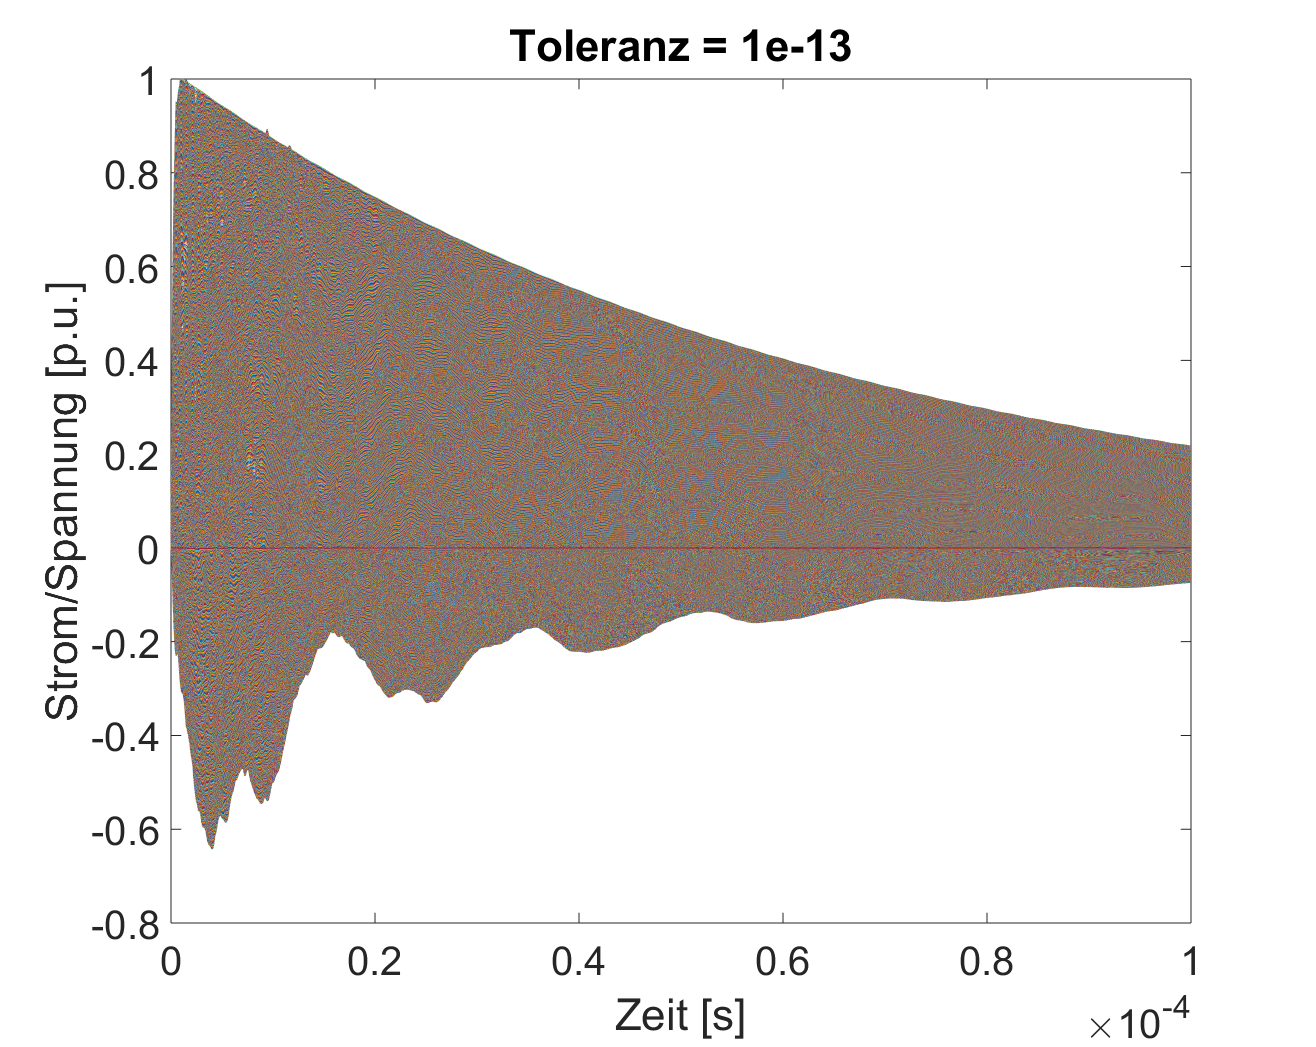
\includegraphics[width=\linewidth]{./trafo/images/svd13.png}
	    \end{minipage}%
	    \begin{minipage}{.5\textwidth}
	        \centering
	        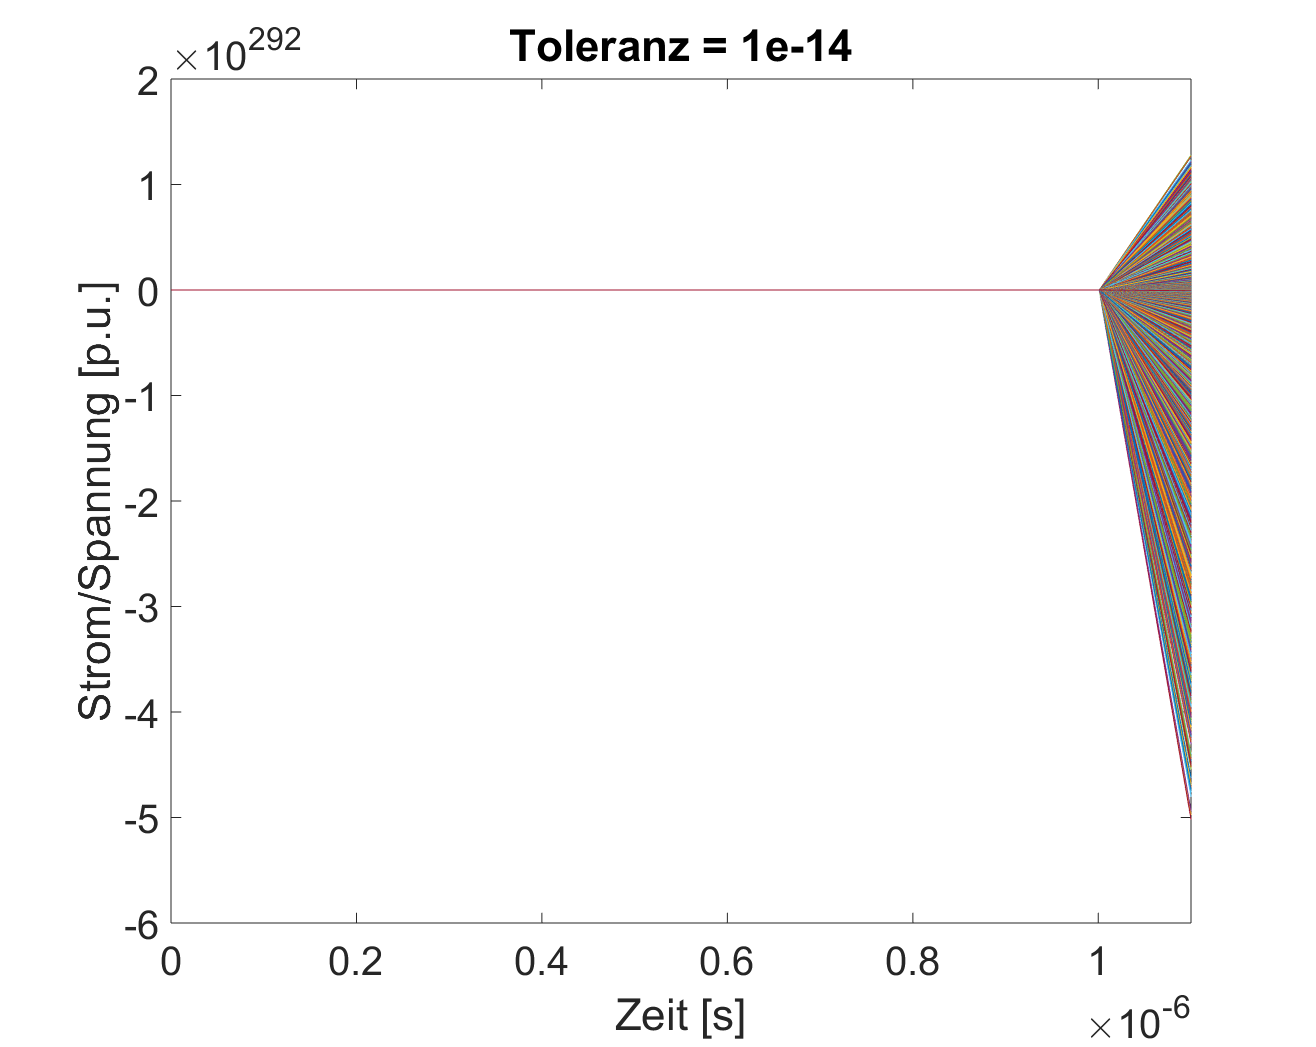
\includegraphics[width=\linewidth]{./trafo/images/svd14.png}
	    \end{minipage}
	    \caption{Numerische Berechnungen mit verschiedenen Toleranzen. Abgebildet sind Str"ome und Spannungen s"amtlicher Windungen. In der Abbildung unten rechts ist ersichtlich, dass die L"osungen bei einer zu klein gew"ahlten Toleranz explodieren und die L"osungen divergieren (es sei auf die Skala der y-Achse hingewiesen). }
	    \label{trafo:SVDTol}
	\end{figure}

\subsection{Exaktes L"osungsverfahren}
\color{red}TODO\color{black}

\subsection{Schrittweite und Fehlerterm}
\color{red}TODO\color{black}

	\begin{figure}
	    \centering
	    \begin{minipage}{.32\textwidth}
	        \centering
	        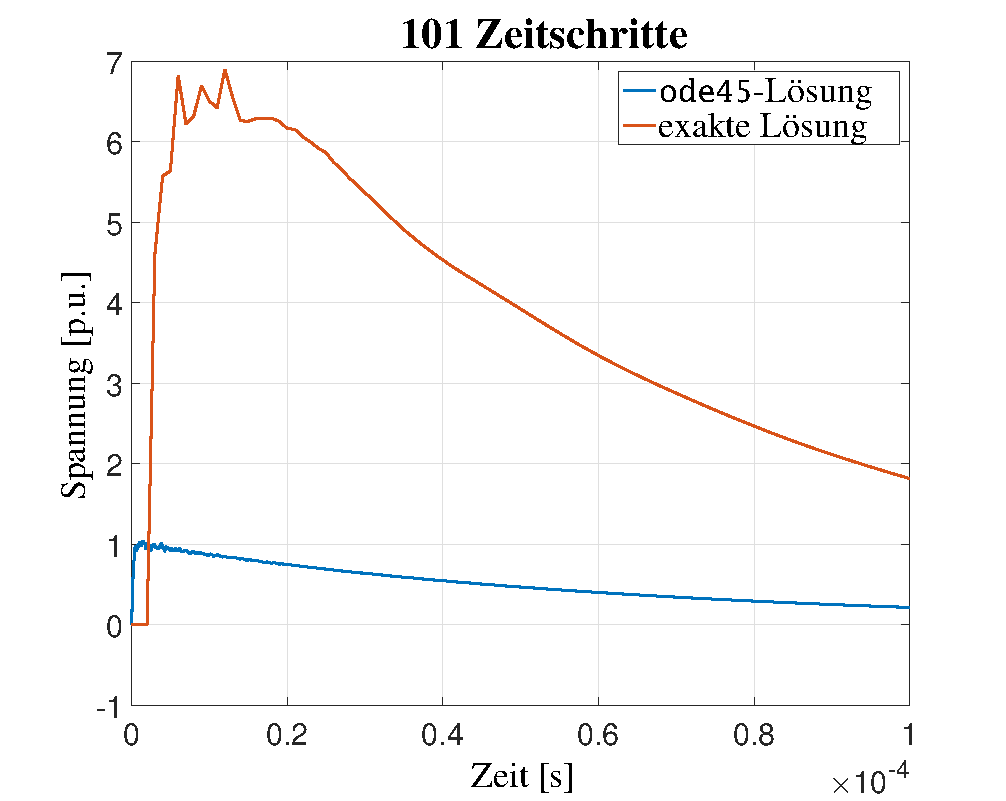
\includegraphics[width=\linewidth]{./Trafo/images/Sprung101.pdf}
	    \end{minipage}%
	    \begin{minipage}{.32\textwidth}
	        \centering
	        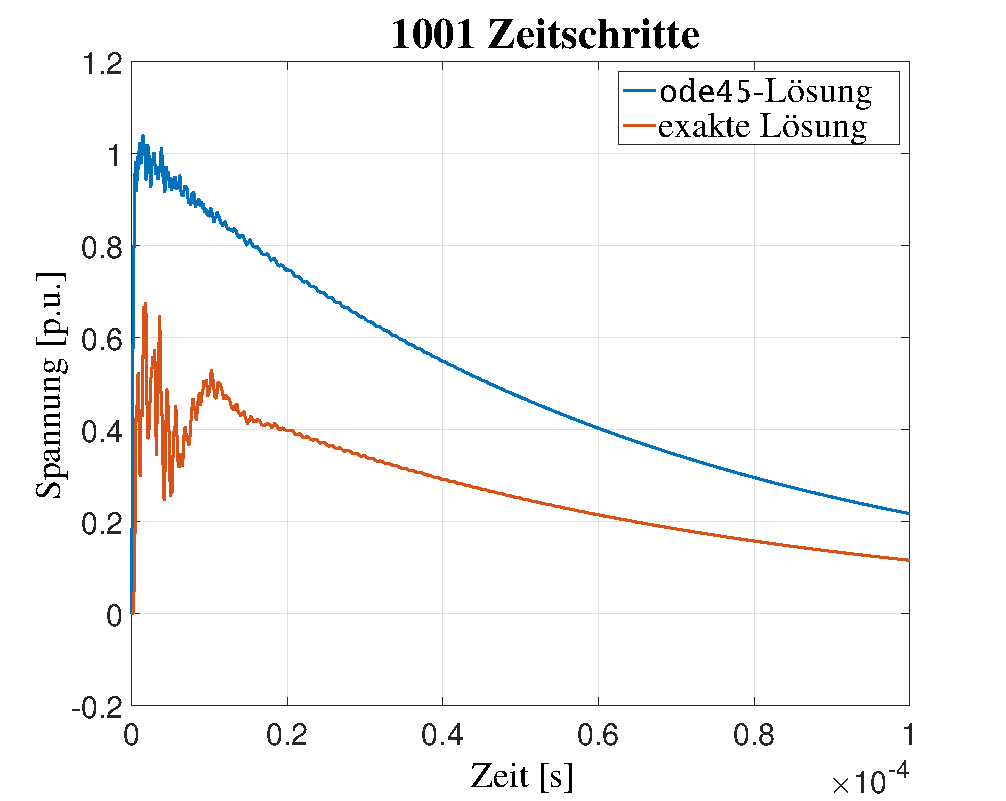
\includegraphics[width=\linewidth]{./Trafo/images/Sprung1001.pdf}
	    \end{minipage}
	    \begin{minipage}{.32\textwidth}
	        \centering
	        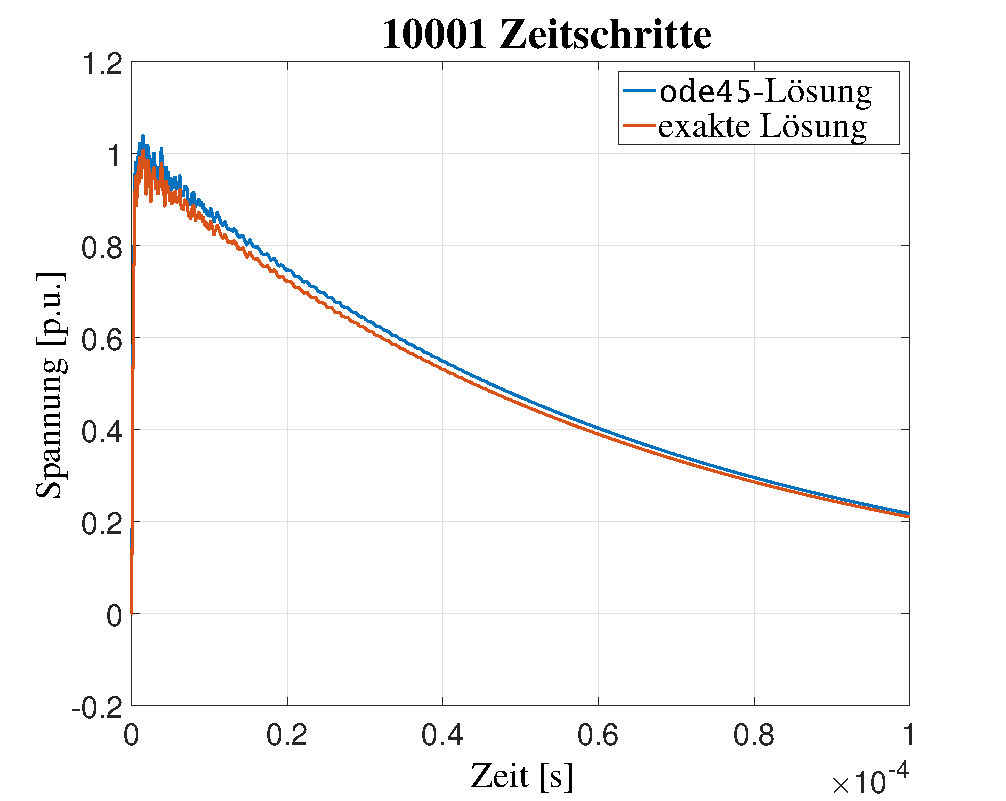
\includegraphics[width=\linewidth]{./Trafo/images/Sprung10001.pdf}
	    \end{minipage}
		\begin{minipage}{.32\textwidth}
	        \centering
	        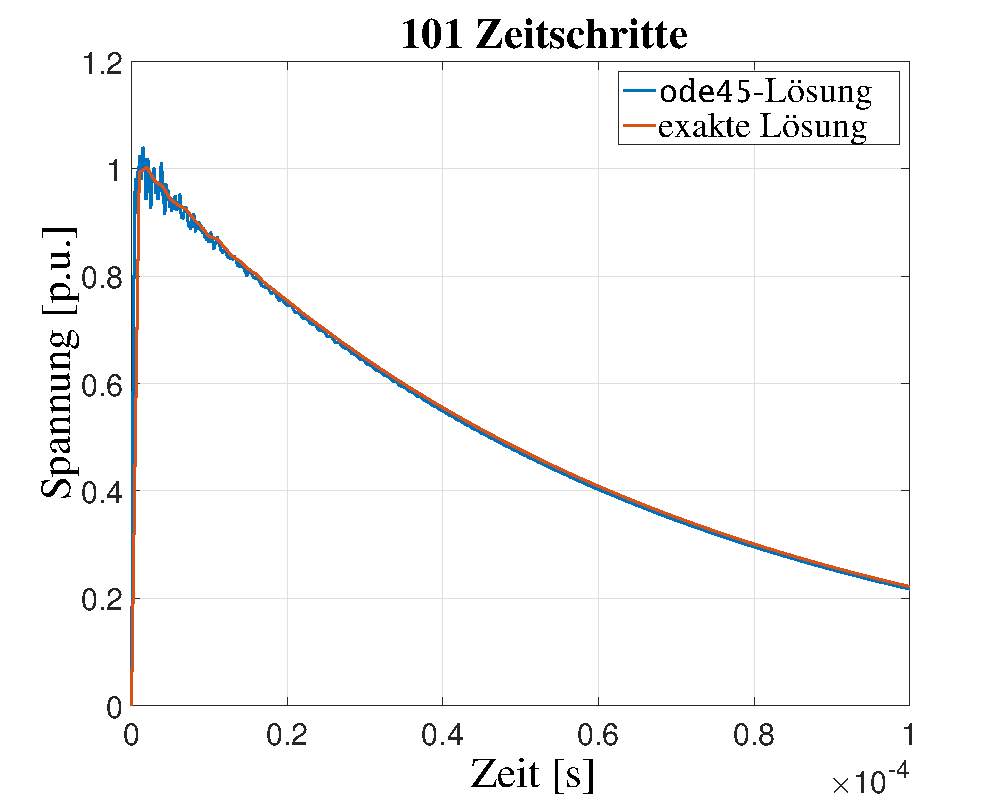
\includegraphics[width=\linewidth]{./Trafo/images/Interp101.pdf}
	    \end{minipage}%
	    \begin{minipage}{.32\textwidth}
	        \centering
	        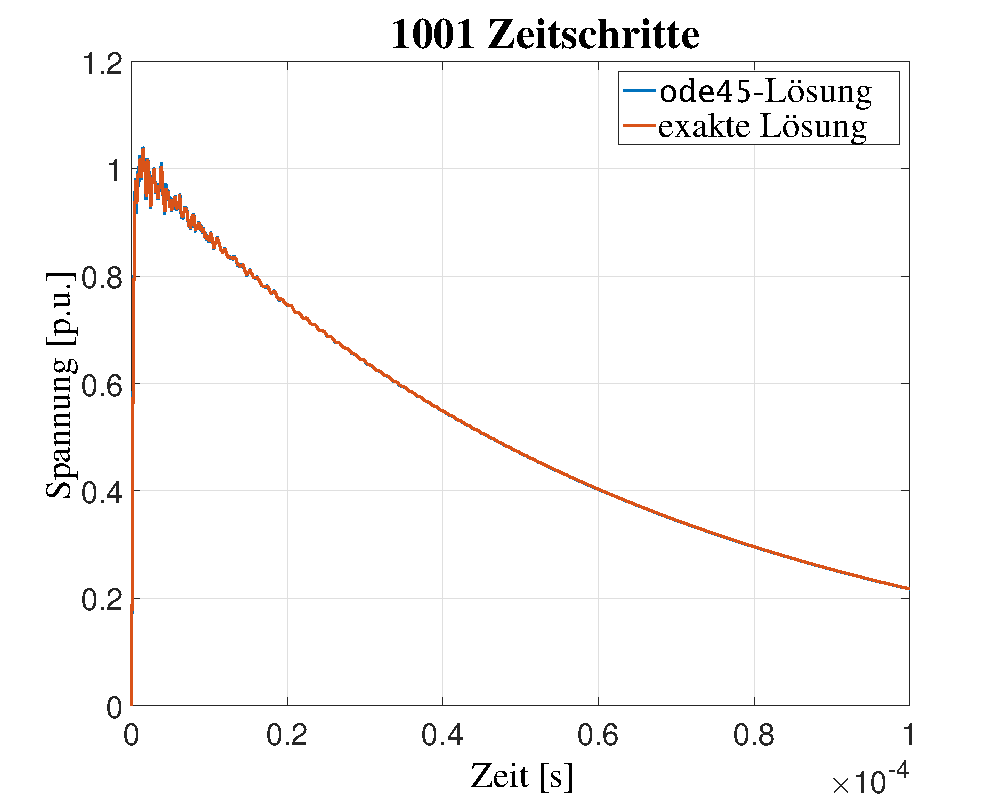
\includegraphics[width=\linewidth]{./Trafo/images/Interp1001.pdf}
	    \end{minipage}
	    \begin{minipage}{.32\textwidth}
	        \centering
	        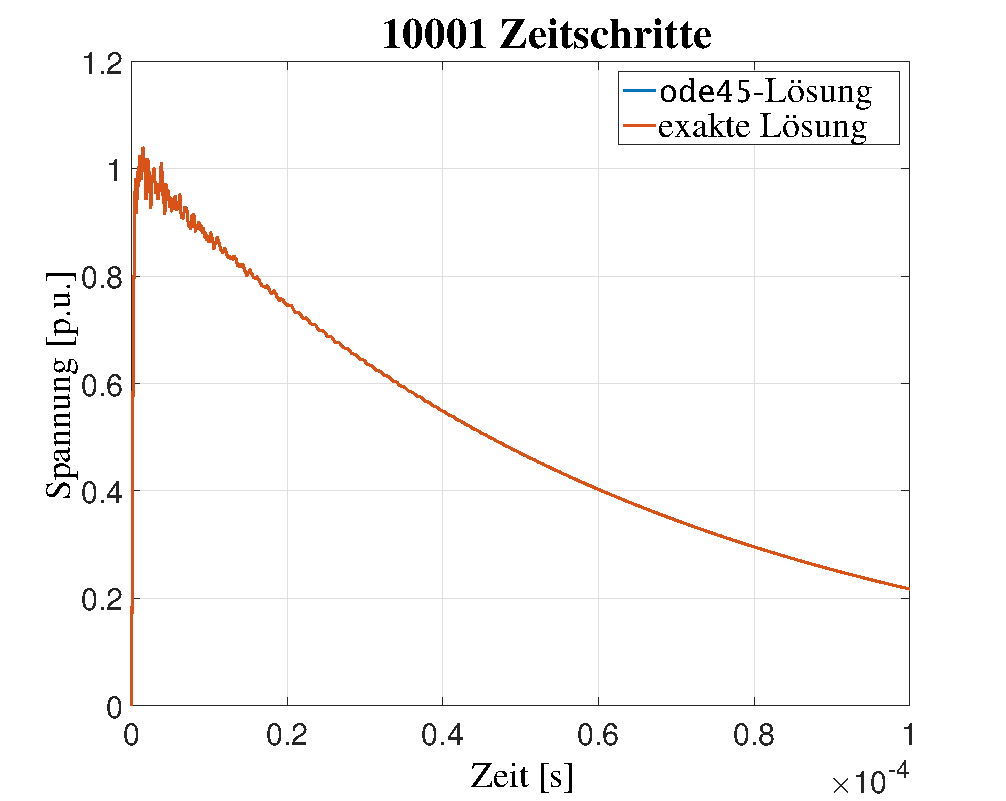
\includegraphics[width=\linewidth]{./Trafo/images/Interp10001.pdf}
	    \end{minipage}
	    \caption{Unterschied konstanter und linearer interpolierter Störterm.}
	\end{figure}

	
		\begin{figure}
			\centering
			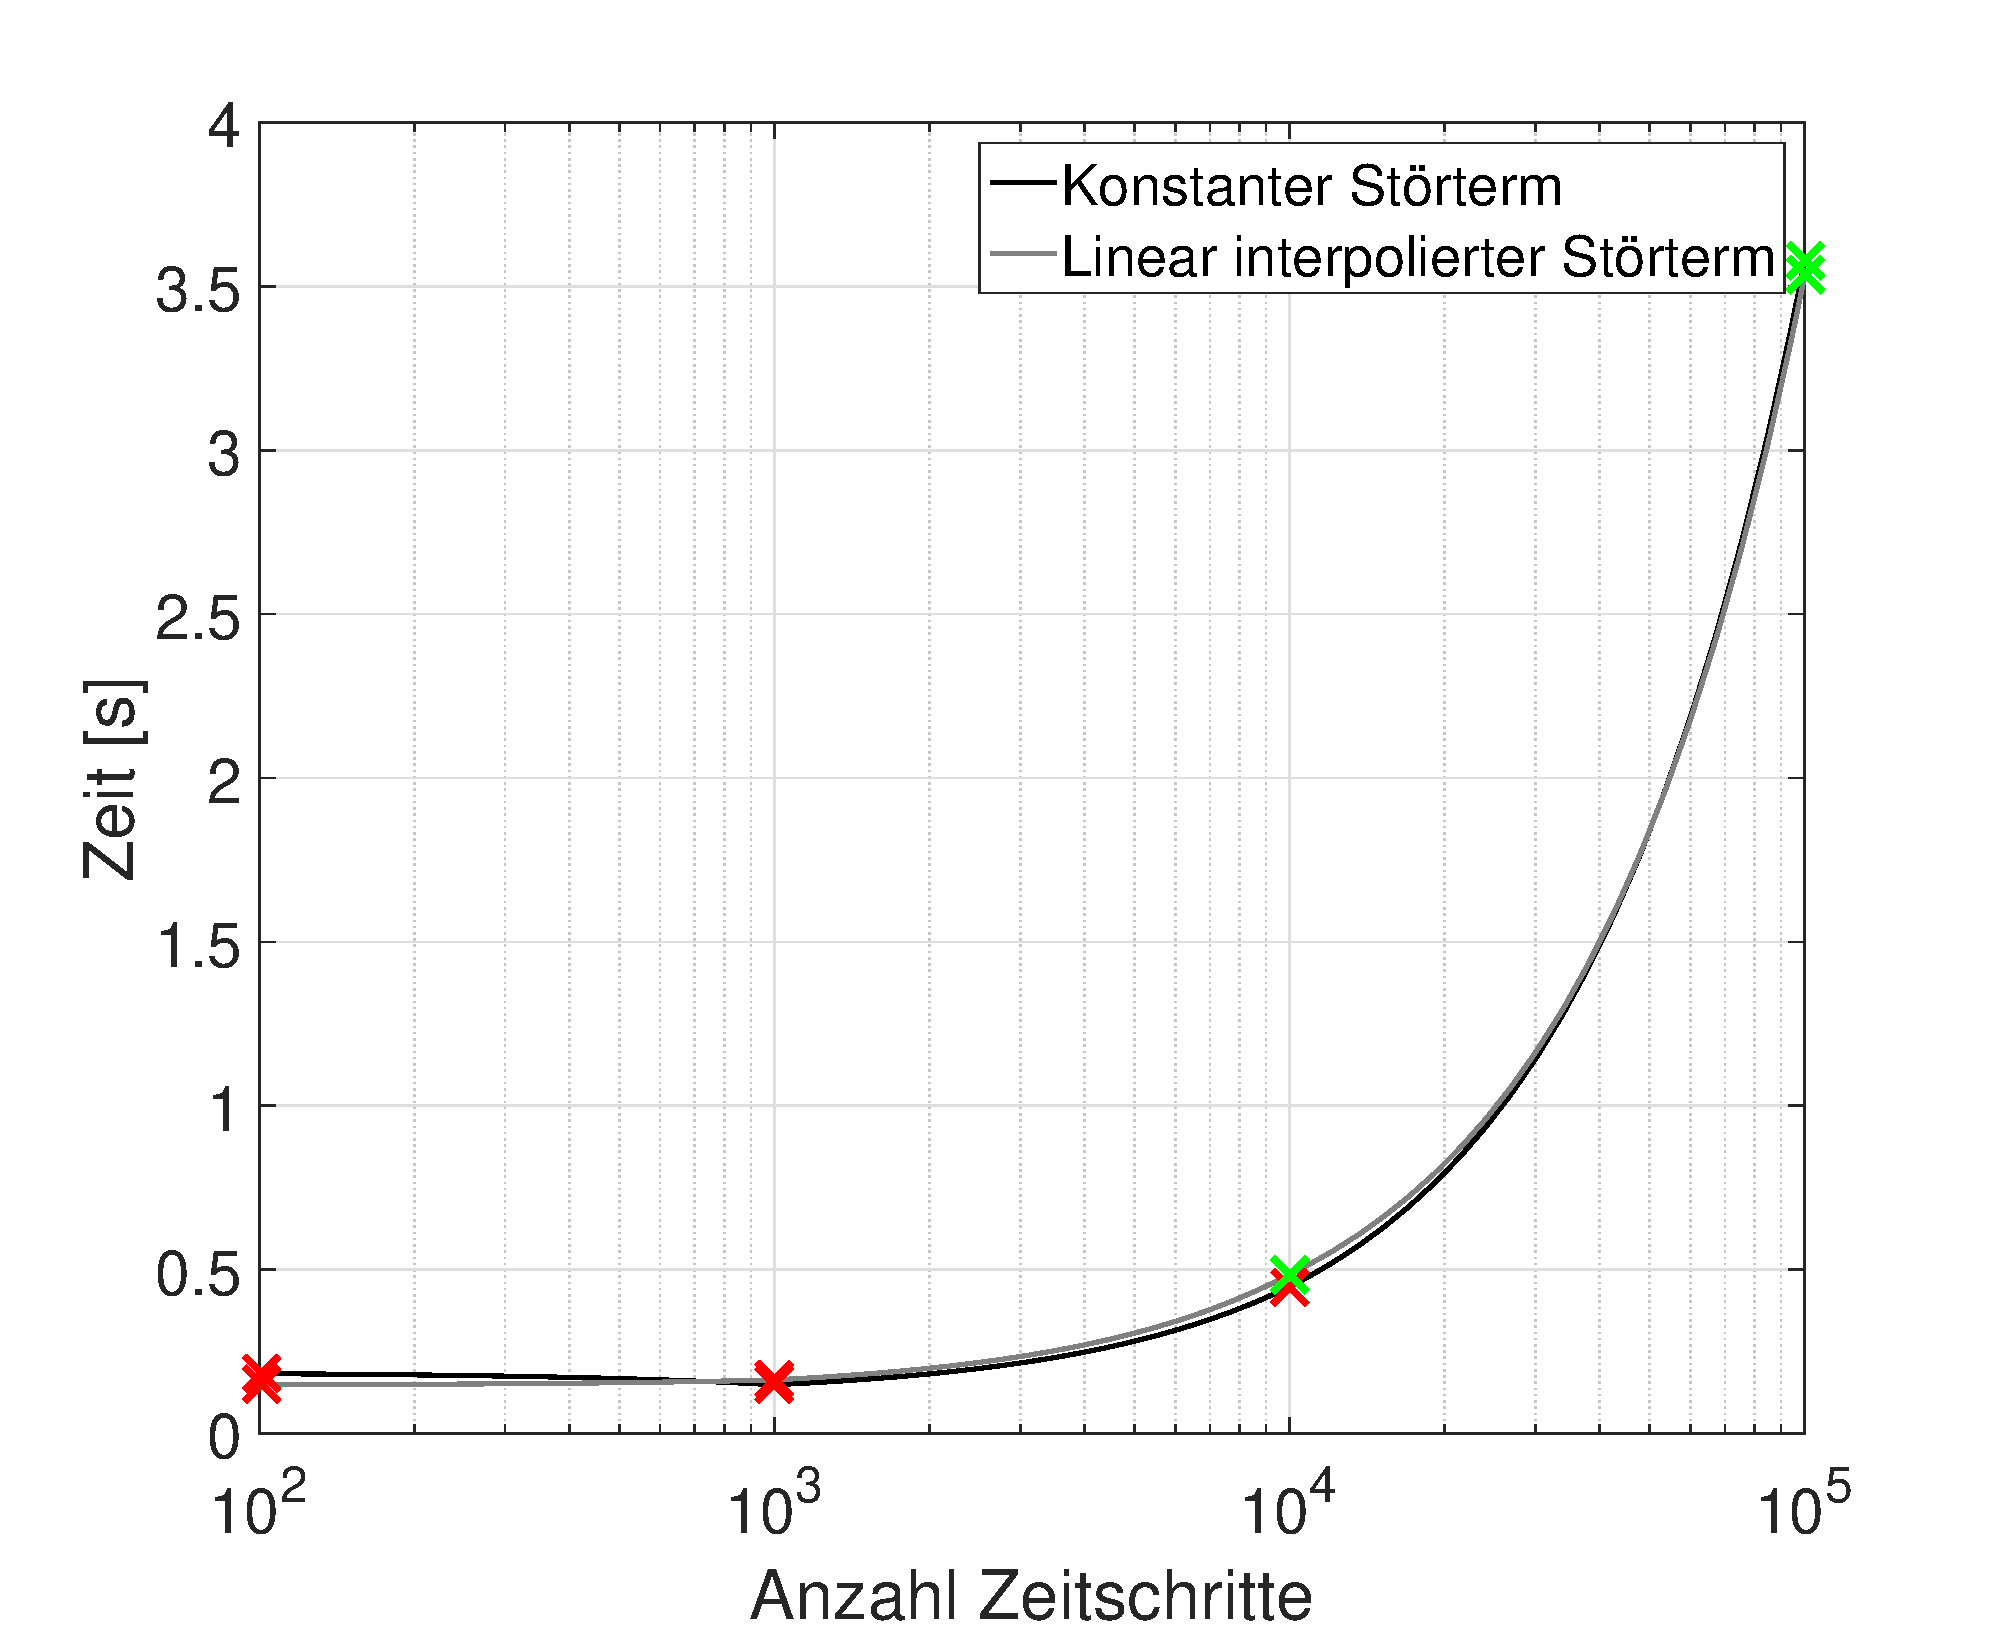
\includegraphics[width=0.9\textwidth]{./Trafo/images/differenceTimestep.pdf}
			\caption{Unterschied konstanter und linearer interpolierter Störterm.}
		\end{figure}
\subsection{Optimierungen}

Ein wichtiger Punkt bei L"osungsverfahren ist die Optimierung. Einen grossen Optimierungsschritt ist bereits beim "Ubergang von der \texttt{ode45}- zur exakten L"osung passiert. Potential zur Verbesserung ist jedoch immer vorhanden.

Der wesentliche Teil der Berechnung, welche beeinflusst werden kann, ist die \textit{for}-Schleife. Diese wird so oft durchlaufen, wie die Anzahl der Schritte gew"ahlt wurde. Deshalb soll das Ziel sein, m"oglichst wenig in dieser Schleife zu berechnen. 

\subsubsection{Exponentialfunktion der Eigenwerte}
Die Gleichung \ref{trafo:exakteLoesung} besitzt eine Konstante $e^{-\Lambda \cdot \Delta t}$, welche bei jedem Zeitschritt mit den neuen Anfangswerten multipliziert wird. Es macht also Sinn, diese Konstante einmal vor der Schleife zu berechnen und als Variable abzuspeichern. Da es sich bei der Matrix $\Lambda$ um eine Diagonalmatrix handelt, h"alt sich auch der Speicherbedarf der Konstante in Grenzen (es sind dies $2n + 1$ Variablen in einer \textit{sparse}-Matrix). 

\subsubsection{Lineare Interpolation}
Die soeben vorgestellte lineare Interpolation \ref{trafo:linInterp} kann mittels Umformungen in die Darstellung 

\begin{equation*}
	y_1 = y_0 \cdot e^{\lambda \cdot \Delta t} + f_0 \underbrace{\left(\left(\frac{e^{\lambda \cdot \Delta t}}{\lambda} - \frac{e^{\lambda \cdot \Delta t}}{\Delta t \cdot \lambda ^2}\right) + \frac{1}{\Delta t \cdot \lambda^2}\right)}_{a_0} + f_1 \underbrace{\left(\frac{e^{\lambda \cdot \Delta t}}{\Delta t \cdot \lambda^2} - \frac{1}{\lambda} - \frac{1}{\Delta t \cdot \lambda^2}\right)}_{a_1}
\end{equation*} 

gebracht werden. Die Konstanten $a_0$ und $a_1$ k"onnen wiederum vor der Schleife einmal berechnet werden. 

Die lineare Interpolation kann jetzt als 
\begin{equation*}
	y_1 = y_0 \cdot e^{\lambda \cdot \Delta t} + a_0 \cdot f_0 + a_1 \cdot f_1
\end{equation*}
geschrieben werden. 

Da sich bei diesem Problem nur die Eingangspannung "andert, ist die Ver"anderung vom transformiertem Vektor $f_0$ zu $f_1$ f"ur alle Elemente dieselbe Zahl $f$. Die Interpolation kann noch etwas einfacher als
\begin{equation*}
	y_1 = y_0 \cdot e^{\lambda \cdot \Delta t} + (a_0 + f \cdot  a_1) \cdot f_0
\end{equation*}
geschrieben werden, wenn $f$ die Differenz der zwei Vektoren $f_0$ und $f_1$ ist. 

\subsubsection{Implementation}
Der Matlab-Code kann jetzt folgendermassen geschrieben werden.

{\scriptsize \lstinputlisting{./trafo/code/compact.m}}


\subsubsection{Vergleich}

Um die Performance zu testen, wird eine sehr schlechte Implementation gew"ahlt, welche eine lineare Interpolation besitzt. Im Gegensatz zum soeben gezeigten Code werden in dieser schlechten Variante alle Konstante in der \textit{for}-Schleife berechnet. Jeder einzelner Zeitschritt dauert bei dieser Berechnung ca. \SI{130}{\milli\second}. 

Als Vergleich wird die schnellste Optimierung verwendet (Matlab-Code von oben). Die Berechnungszeit f"ur jeden einzelnen Zeitschritt konnte bis auf \SI{35}{\micro \second} reduziert werden. 

Die Grafik \ref{trafo:Optimierung} zeigt den Unterschied in einer doppelt logarithmischen Grafik. Die Optimierungsversuche haben sich auch in der Praxis als hervorragend erwiesen.

\begin{figure}
	\centering
	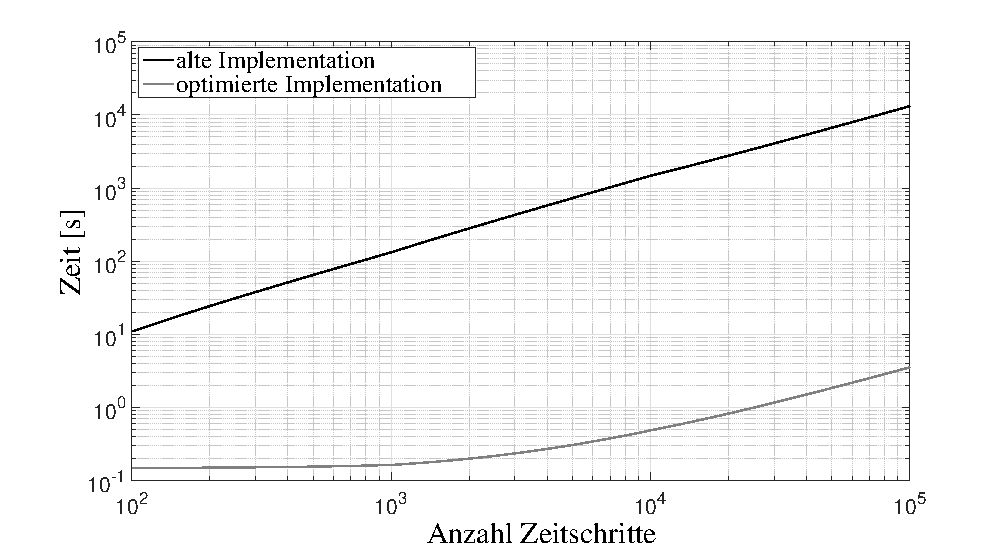
\includegraphics[width=0.9\textwidth]{./trafo/images/differenceOptimization.pdf}
	\caption{Unterschied zwischen einer sehr schlechten und einer guten Implementierung bei einem Trafomodell mit 500 Windungen.}
	\label{trafo:Optimierung}
\end{figure}

\subsection{Vergleich zwischen numerischer und exakter L"osung}
\color{red}TODO\color{black}

	\begin{figure}
		\centering
		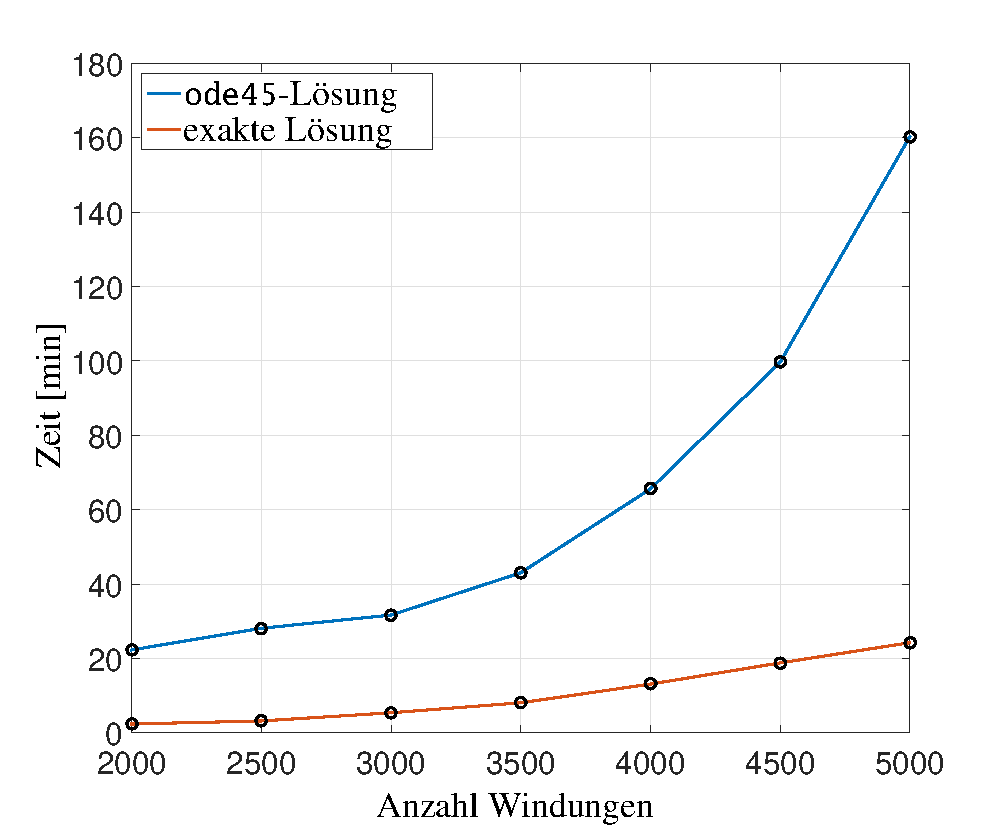
\includegraphics[width=0.6\textwidth]{./Trafo/images/ode45vsExact.pdf}
	\end{figure}

\section{Anwendung der gefundenen L"osungen}

Schlussendlich k"onnen die gefundenen L"osungen wieder in das CAD-Modell eingelesen werden, damit das elektrische Feld simuliert werden kann. Somit kann festgestellt werden, wo sich Schwachstellen im Transformator befinden und diese allenfalls verbessert werden.

Interessant ist nat"urlich immer der gr"osste Spannungsunterschied zwischen benachbarten Wicklungen. In diesem Beispiel ist dies zwischen dem Layer 1 und 2 zwischen Wicklung 6 und 118.

Diese L"osung wurde bereits in Abbildung \ref{trafo:loesung} pr"asentiert. Das elektrische Feld zum Zeitpunkt der gr"ossten Spannungsdifferenz ist in den Abbildungen \ref{trafo:E-Field} und \ref{trafo:E-FieldZoom} dargestellt. 

\begin{figure}
	\centering
	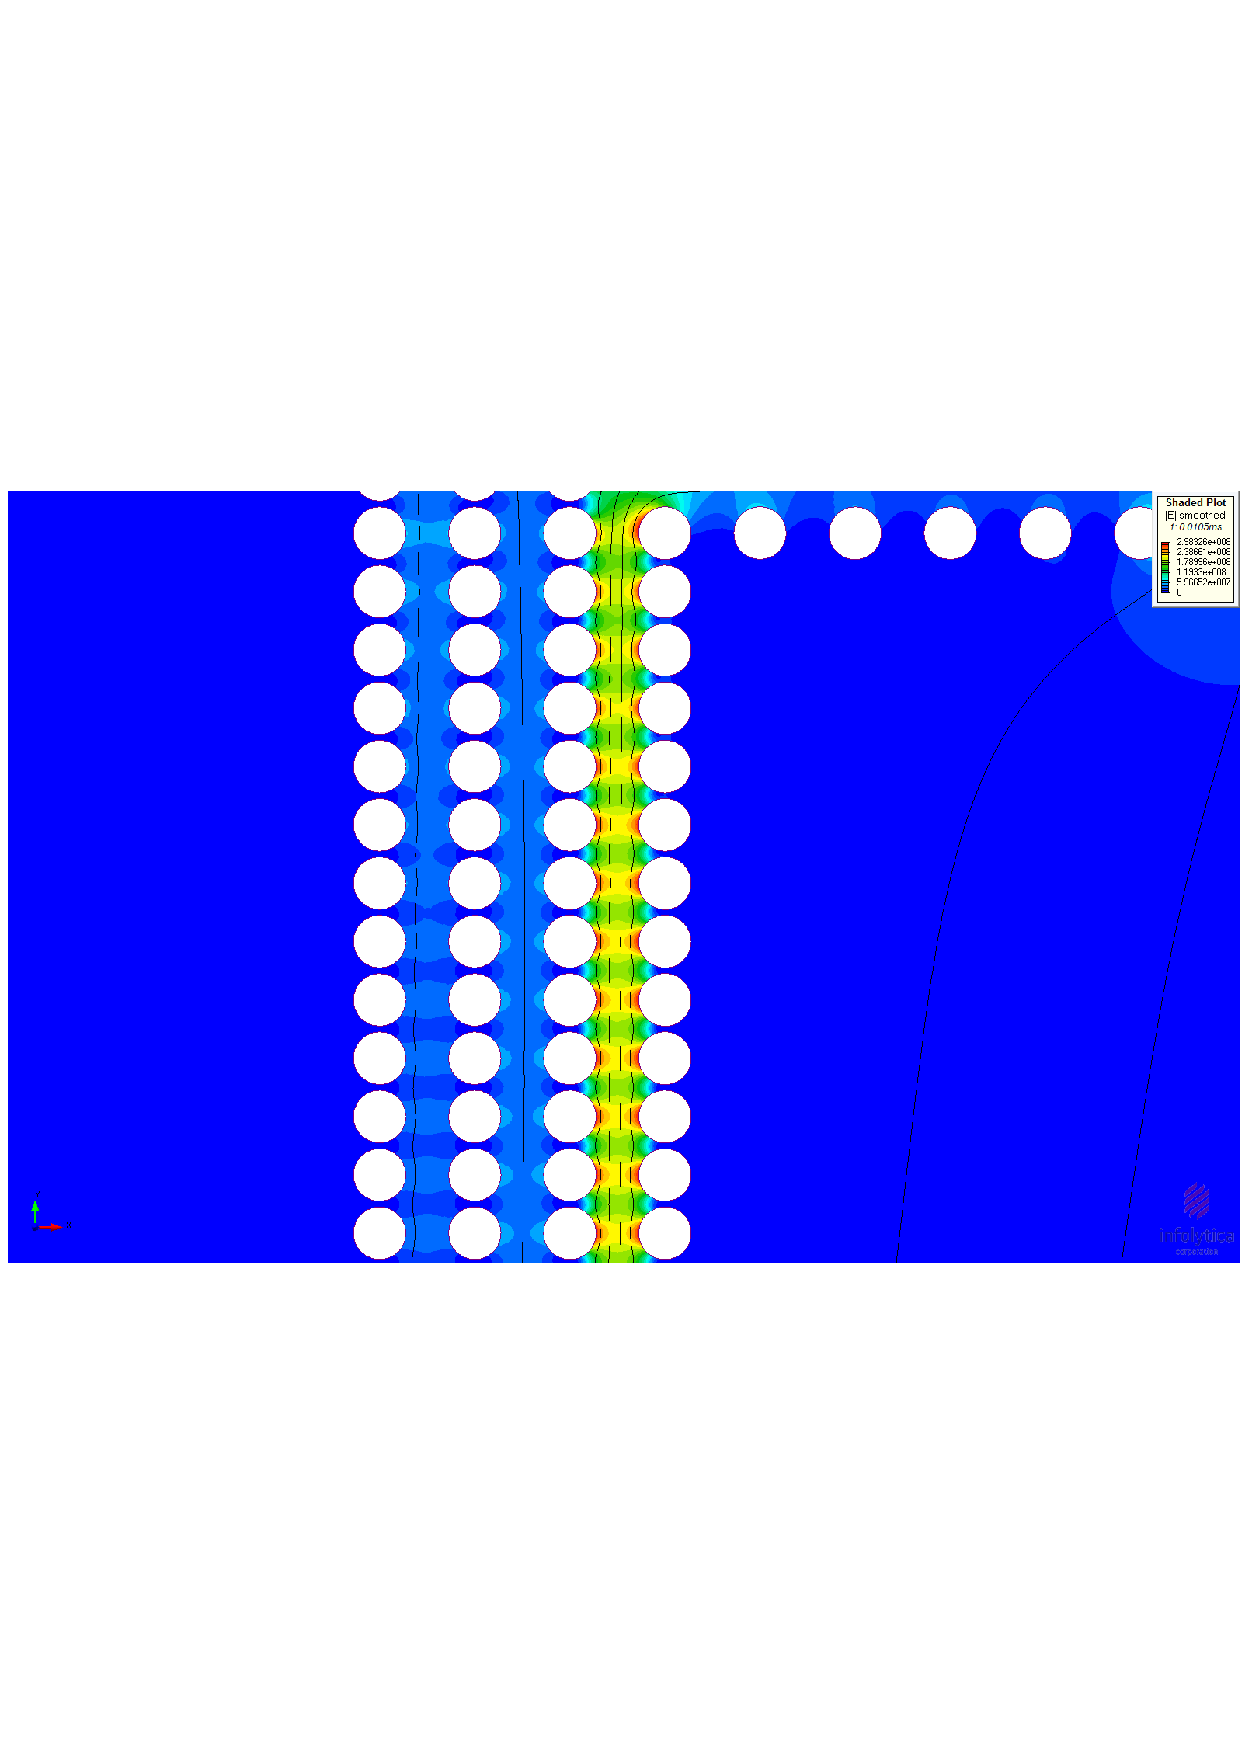
\includegraphics[width=\textwidth]{./trafo/images/BIL_VoltageTrans.pdf}
	\caption{Elektrisches Feld zwischen den ersten paar Layern.}
	\label{trafo:E-Field}
\end{figure}

\begin{figure}
	\centering
	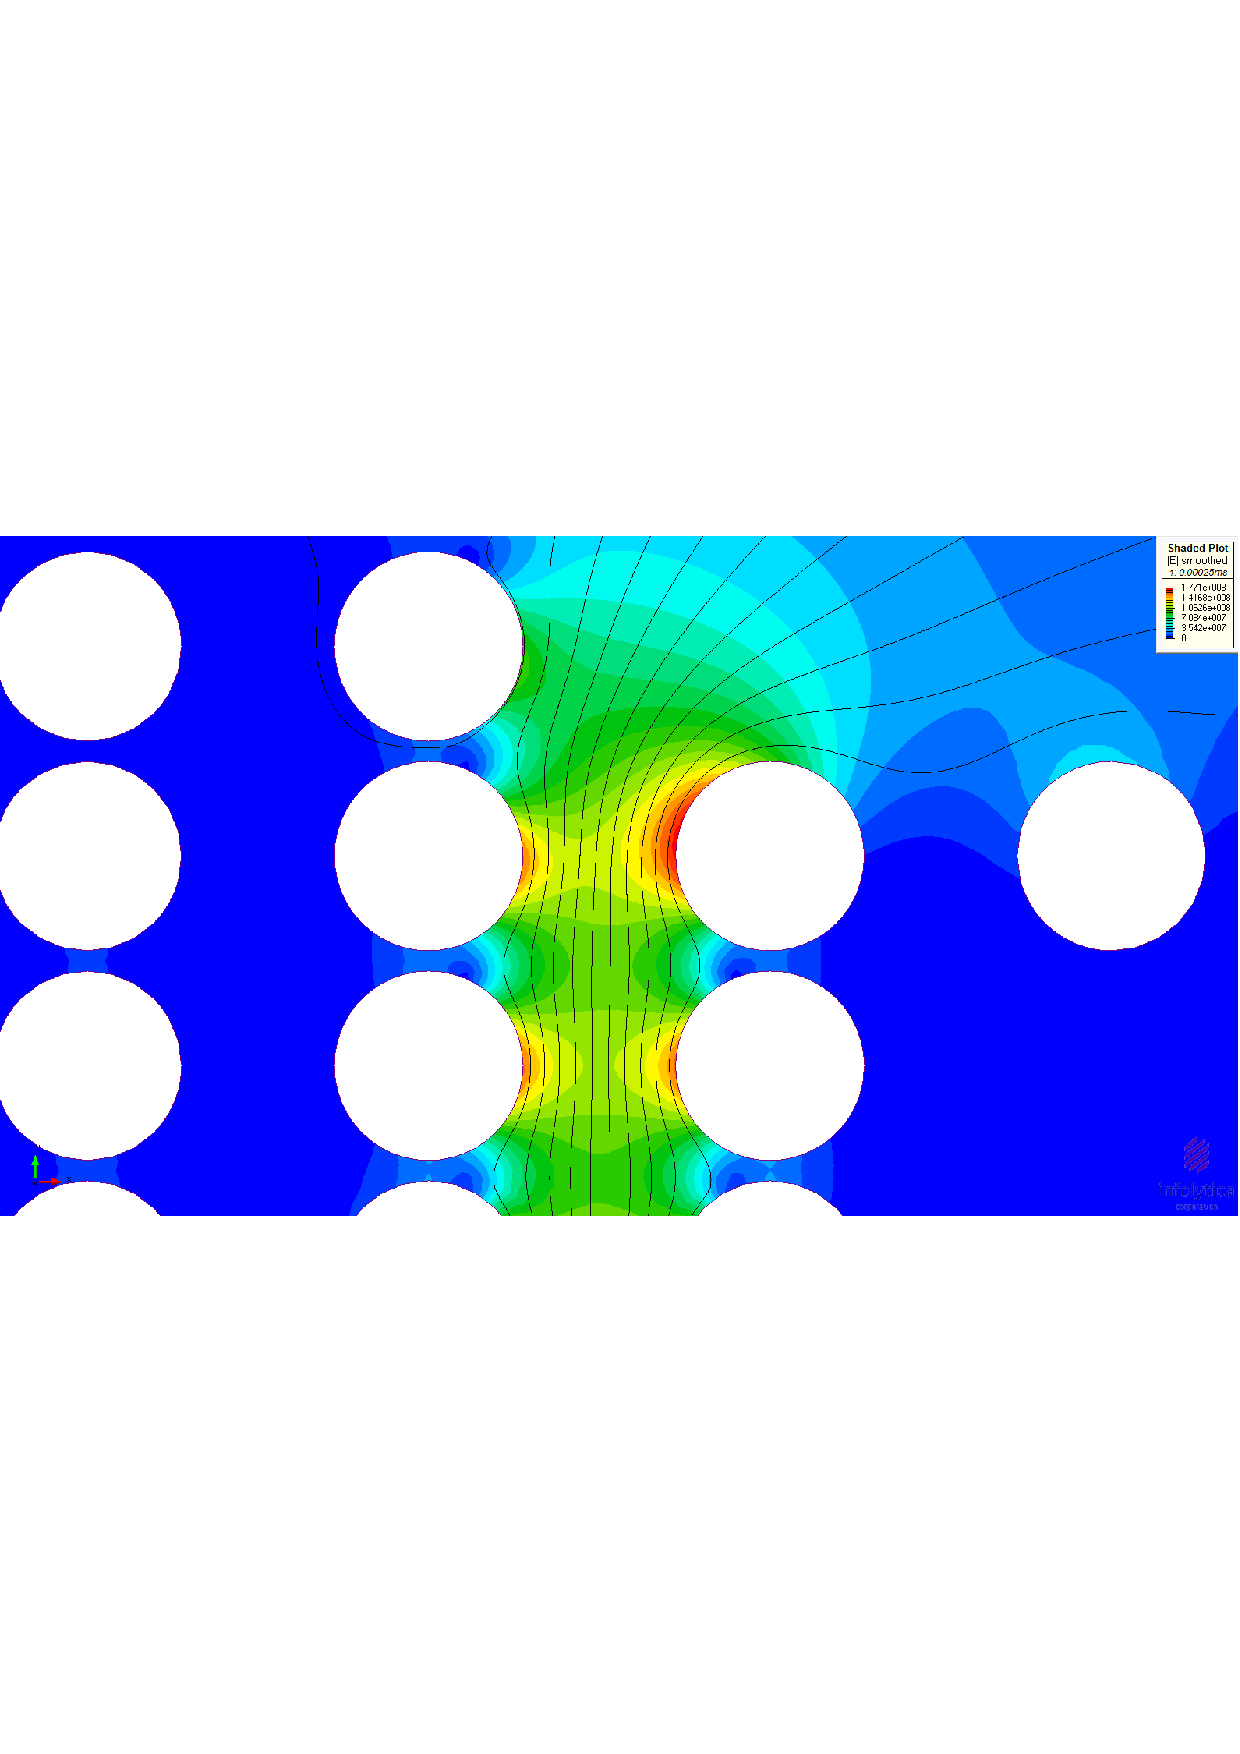
\includegraphics[width=\textwidth]{./trafo/images/VoltageTrans.pdf}
	\caption{Elektrisches Feld zwischen Windung 6 und 118.}
	\label{trafo:E-FieldZoom}
\end{figure}

Da die Herstellung von Transformatoren nie optimal abl"auft, k"onnen sich auch Luftblasen im Epoxidharz bilden. Diese Luftblasen, auch Lunker genannt, verst"arken das elektrische Feld zus"atzlich und schw"achen somit den Transformator im Fehlerfall. Ein m"ogliches Szenario ist in Abbildung \ref{trafo:E-FieldBubble} pr"asentiert. 

\begin{figure}
	\centering
	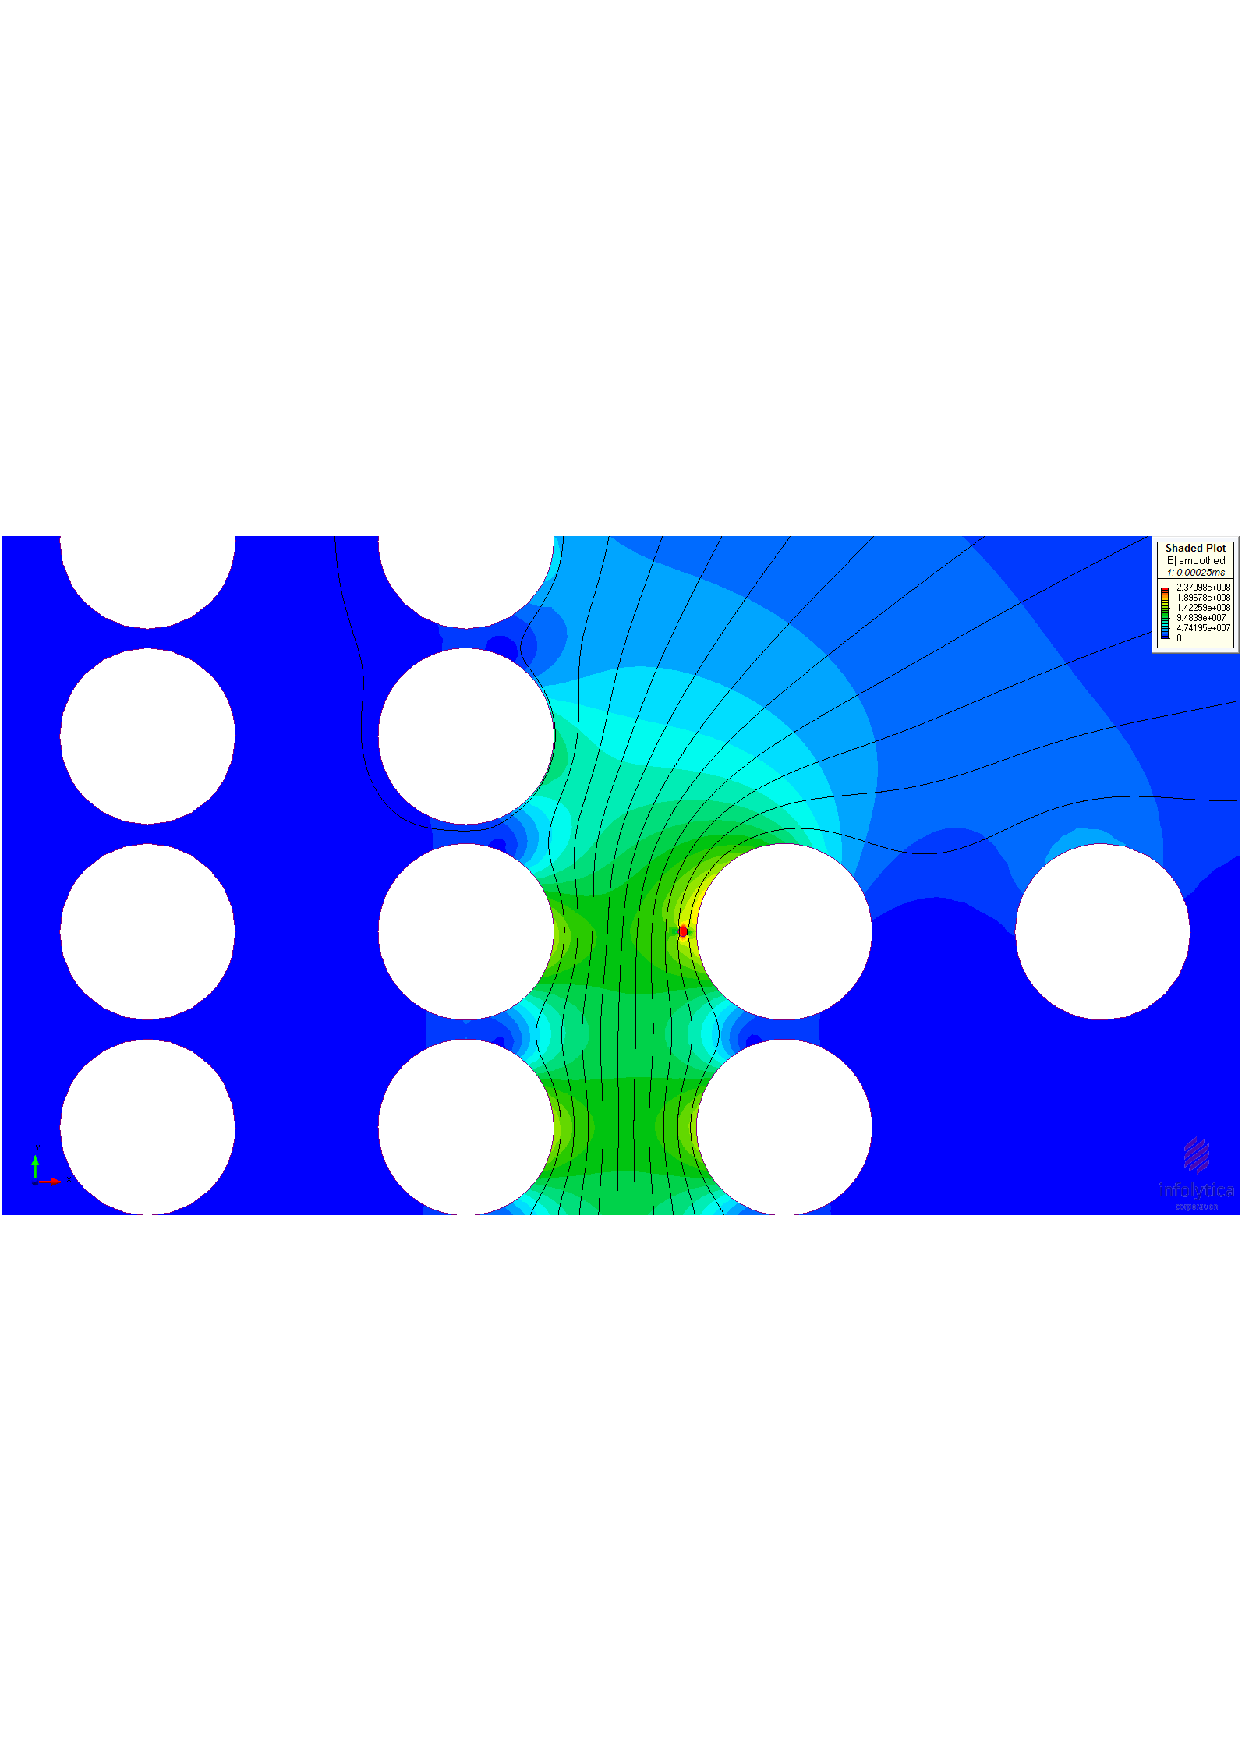
\includegraphics[width=\textwidth]{./trafo/images/VoltageTrans_bubble_turn6_10u_9u.pdf}
	\caption{Elektrisches Feld zwischen Wicklung 6 und 118 mit simulierter Luftblase (Lunker).}
	\label{trafo:E-FieldBubble}
\end{figure}

\subsection{Schlussfolgerung}
Das Problem kann erfolgreich formuliert werden und automatisiert werden. Mit mathematischen Hilfsmitteln ist es auch m"oglich, grosse Matrizen zu berechnen. \color{red} TODO \color{black}

\printbibliography[heading=subbibliography]
\end{refsection}
